\chapter{Как быстро идут химические реакции}

\section{Что такое скорость реакции}

В предыдущей главе мы разобрались, при каких условиях химическая реакция является самопроизвольной, а при каких будет протекать обратный процесс. При этом термодинамика совершенно не отвечает на вопрос \emph{как быстро будет происходить реакция}. Из своего жизненного опыта вы знаете, что некоторые реакции происходят практически мгновенно (например, взрыв), иногда в течение нескольких минут (горение древесины), иногда в течение нескольких лет (ржавление железа), а иногда и целых эпох (выветривание горных пород).

Однако для точной науки слов <<быстро>> и <<медленно>> недостаточно, нужны числовые значения. Вы уже встречали знак $\tau$ над стрелкой в уравнении реакции (табл.~\ref{tab:designation_of_reaction_conditions}), который показывает, что реакции требуется время. Теперь мы научимся определять, сколько именно.

В этой главе мы постараемся ответить на три главных вопроса:

\begin{itemize}
    \item как количественно описать, насколько быстро идёт реакция;
    \item от чего зависит скорость реакции и как ею управлять;
    \item может ли скорость реакции рассказать о её механизме.
\end{itemize}

Раздел химии, который изучает скорости химических реакций и то, \emph{каким путём} они протекают, называется \term{химической кинетикой}{chemical_kinetics}{химическая кинетика} (от греч. \grk{k'inhsis} (\textit{k\'{\i}n\={e}sis})~--- движение).

\subsection*{О скорости}

\emph{Скорость}~--- это изменение, происходящее за определённый промежуток времени. Например, скорость автомобиля принято определять в количестве километров, которые он проезжает за один час. Банковскую ставку (это тоже скорость) определяют как количество процентов от суммы вашего вклада, на которые увеличится ваша сумма за один год. Таким образом, в общем виде

\begin{equation}
    \label{eq:definition_of_speed}
    \text{Скорость} = \frac{\text{Изменение}}{\text{Промежуток времени}}.
\end{equation}

Когда мы говорим о скорости химической реакции, то логично использовать изменение количеств (концентраций) веществ в ходе реакции. При этом концентрация исходных веществ будет уменьшаться, а продуктов~--- расти.

В зависимости от того, какую химическую систему мы рассматриваем, числитель выражения \eqref{eq:definition_of_speed} можно выразить в любых величинах, отражающих изменение количеств веществ в реакции, например, в виде изменения \emph{концентрации вещества} (в случае растворов), \emph{парциального давления} (в случае газов это эквивалентно концентрации), \emph{единиц длины} (при рассмотрении глубины коррозии), просто в молях и т.~п.

\subsection*{Кинетическая кривая}

Для изучения скорости реакции наиболее удобно представить величины, связанные с изменением количеств веществ, в виде графика зависимости от времени. Такой график называют \term{кинетической кривой}{kinetic_curve}{кинетическая кривая}. Для построения такого графика сначала строят таблицу, измеряя концентрации веществ через определённые промежутки времени, а затем наносят эти точки на график. Например, в таблице~\ref{tab:ethanol_in_blood} представлены концентрации этанола в крови человека после внутривенного введения, а на рис.~\ref{fig:ethanol_in_blood}~--- кинетическая кривая, построенная на её основе.

\begin{table}[htbp]
    \small
    \caption{Концентрация этанола в крови человека после внутривенного введения.}
    \label{tab:ethanol_in_blood}
    \begin{tabularx}{\textwidth}{
        >{\hsize=1\hsize}Z
        >{\hsize=1\hsize}Z
        >{\hsize=1\hsize}Z
        }
        \hline
        \rowcolor{table_header}
        $t$, \unit{\ruCh} & $c(\ce{C2H5OH})$, \unit{\ruMmole\per\ruL} & $c(\ce{C2H5OH})$, \unit{\ruG\per\ruL} \\
        \hline
        0 & \num{35,0} & \num{1,61} \\
        1 & \num{31,7} & \num{1,46} \\
        2 & \num{28,4} & \num{1,31} \\
        3 & \num{25,1} & \num{1,16} \\
        4 & \num{21,8} & \num{1,00} \\
        5 & \num{18,5} & \num{0,85} \\
        6 & \num{15,2} & \num{0,70} \\
        7 & \num{11,9} & \num{0,55} \\
        8 & \num{8,6} & \num{0,40} \\
        9 & \num{5,3} & \num{0,24} \\
        \hline
    \end{tabularx}
\end{table}

\begin{figure}[htbp]
    \centering
    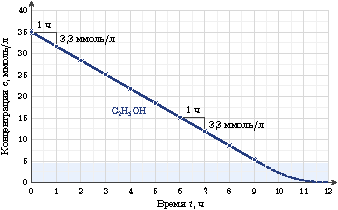
\includegraphics[width=12cm]{figs/what_is_reaction_rate/ethanol_zero_order.pdf}
    \caption{График на основании таблицы~\ref{tab:ethanol_in_blood}.}
    \label{fig:ethanol_in_blood}
\end{figure}

Как мы видим, концентрация этанола в крови изменяется линейно, равномерно убывая через равные промежутки времени, исключая период, когда этанол почти полностью метаболизирован.

Однако кинетическая кривая не всегда является линейной. Давайте рассмотрим изученную в 1930~году Эйрингом и Даниэлсом реакцию разложения при \qty{45}{\degreeCelsius} оксида азота (V)\footnote{H. Eyring, F. Daniels. J. Am. Chem. Soc. 52, 1472 (1930), табл. II, опыт 2.}, растворённого в \ce{CCl4}:

\reaction[ce:n2o5_decomposition]{2N2O5 -> 2N2O4 + O2 (^) {.}}

Тетраоксид диазота \ce{N2O4} остаётся в растворе, а кислород выделяется из него в виде газа\footnote{Сначала образуется диоксид азота в ходе реакции \ce{2N2O5 -> 4NO2 + O2}. Затем, как вы помните из задачи~\ref{prob:gibbs_energy2}, молекулы \ce{NO2} объединяются в \ce{N2O4}, поэтому уравнение записано сразу с \ce{N2O4}. Тем не менее раствор всё равно будет выглядеть бурым из-за небольшого количества \ce{NO2}.}. Концентрацию \ce{N2O5} определяли в разные моменты времени, результаты показаны в табл.~\ref{tab:n2o5_decomposition}\footnote{В статье для каждого момента времени указан объём кислорода, который \emph{ещё выделится} до конца реакции. Этот объём пропорционален количеству оставшегося \ce{N2O5}, по нему вычисляется концентрация \ce{N2O5}, а концентрации \ce{N2O4}~--- по уравнению~\eqref{ce:n2o5_decomposition}.}.

\begin{table}[htbp]
    \small
    \caption{Разложение \ce{N2O5} в растворе в \ce{CCl4} при \qty{45}{\degreeCelsius}.}
    \label{tab:n2o5_decomposition}
    \begin{tabularx}{\textwidth}{
        >{\hsize=1\hsize}Z
        >{\hsize=1\hsize}Z
        >{\hsize=1\hsize}Z
        }
        \hline
        \rowcolor{table_header}
        $t$, с & $c(\ce{N2O5})$, \unit{\ruMole\per\ruL} & $c(\ce{N2O4})$, \unit{\ruMole\per\ruL} \\
        \hline
        0 & \num{2,33} & 0 \\
        \num{184} & \num{2,07} & \num{0,26} \\
        \num{319} & \num{1,91} & \num{0,42} \\
        \num{526} & \num{1,68} & \num{0,65} \\
        \num{867} & \num{1,35} & \num{0,98} \\
        \num{1198} & \num{1,11} & \num{1,22} \\
        \num{1877} & \num{0,72} & \num{1,61} \\
        \hline
    \end{tabularx}
\end{table}

Построим кинетические кривые для реагента и основного продукта (рис.~\ref{fig:kinetic_curves}). Поскольку реагент расходуется в реакции, то его кривая идёт вниз, а концентрация продукта растёт (кривая идёт вверх), причём кривые являются взаимным отражением друг друга, потому что по уравнению~\eqref{ce:n2o5_decomposition} на каждую разложившуюся молекулу \ce{N2O5} образуется одна молекула \ce{N2O4}.

\begin{figure}[htbp]
    \centering
    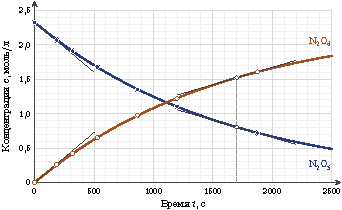
\includegraphics[width=12cm]{figs/what_is_reaction_rate/kinetic_curves.pdf}
    \caption{Кинетические кривые разложения \ce{N2O5} в растворе в \ce{CCl4} при \qty{45}{\degreeCelsius}. Закрашенные точки~--- концентрации \ce{N2O5}, полученные в результате эксперимента, незакрашенные~--- концентрации \ce{N2O4}, вычисленные по уравнению реакции. Отрезками показаны касательные к обеим кривым в начальный момент времени и в момент $t = \qty{1700}{\ruS}$.}
    \label{fig:kinetic_curves}
\end{figure}

Обратите внимание на форму кинетических кривых. В отличие от случая разложения этанола в крови, они не являются линейными. В начальный момент времени концентрации меняются быстро, но чем дольше протекает реакция, тем медленнее это происходит. За первые \qty{526}{\ruS} концентрация \ce{N2O5} упала на \qty{0,65}{\ruMole\per\ruL}, а за \qty{679}{\ruS} между 1198-й и 1877-й секундами~--- всего на \qty{0,39}{\ruMole\per\ruL}, хотя этот промежуток даже длиннее. Другими словами, реакция постепенно замедляется. Это означает, что в данном случае не существует единой скорости на всём времени протекания реакции и можно говорить о скорости только применительно к определённому промежутку или моменту времени.

Почему скорость в данном случае не остаётся постоянной? По мере протекания реакции молекулы \ce{N2O5} расходуются, превращаясь в продукты, и их остаётся всё меньше в одном и том же объёме раствора. При этом в любой момент времени (и в начале, и в конце реакции) вероятность превращения за единицу времени для каждой из оставшихся молекул всегда остаётся той же самой. В данном случае за любые \qty{650}{\ruS} разлагается примерно треть тех молекул \ce{N2O5}, которые были в растворе в начале этого промежутка времени (рис.~\ref{fig:constant_fraction}). В каждом промежутке реагирует треть от всё меньшего числа молекул, поэтому мы видим, как за одно и то же время распадается всё меньше \ce{N2O5}.

\begin{figure}[htbp]
    \centering
    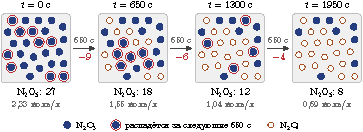
\includegraphics[width=12cm]{figs/what_is_reaction_rate/constant_fraction.pdf}
    \caption{Почему разложение \ce{N2O5} замедляется. Одна и та же порция раствора представлена в моменты \num{0}, \num{650}, \num{1300} и \qty{1950}{\ruS}. 27 молекул соответствуют начальной концентрации \qty{2,33}{\ruMole\per\ruL}. За каждые \qty{650}{\ruS} распадается треть имеющихся молекул \ce{N2O5} (они обведены), но число распадов уменьшается (\num{9}, \num{6} и \num{4}). На месте каждой распавшейся молекулы \ce{N2O5} показана молекула \ce{N2O4}.}
    \label{fig:constant_fraction}
\end{figure}

Почему же, спросите вы, в таком случае скорость распада этанола остаётся одной и той же на протяжении почти всего времени? Дело в том, что этанол в печени окисляется ферментом \emph{алкогольдегидрогеназой}, которого имеется весьма ограниченное количество. Из-за этого скорость зависит просто от того, сколько фермента имеется в организме (каждая молекула фермента оказывается занята процессом, и оставшийся этанол <<ждёт>> своей очереди), а не от концентрации молекул этанола. Когда этанола становится мало, фермент начинает простаивать, и скорость падает~--- это отвечает закрашенной области на рис.~\ref{fig:ethanol_in_blood}.

\subsection*{Средняя скорость}

Скорость реакции на каком-то промежутке времени проще всего описать, разделив изменение концентрации на длительность этого промежутка. В этом случае мы получим \term{среднюю скорость}{average_rate}{средняя скорость} на промежутке времени от $t_1$ до $t_2$. Для реагента A
\begin{equation}
    \label{eq:average_rate}
    \overline{v}(\mathrm{A}) = -\frac{\Delta c(\mathrm{A})}{\Delta t} = -\frac{c_2 - c_1}{t_2 - t_1},
\end{equation}
где $c_1$ и $c_2$~--- его концентрации в моменты $t_1$ и $t_2$. Минус здесь нужен из-за того, что концентрация реагента уменьшается и $\Delta c < 0$ (а скорость принято считать положительной). Для продукта B концентрация растёт, поэтому минус не нужен: $\overline{v}(\mathrm{B}) = \Delta c(\mathrm{B})/\Delta t$.

Скорость, найденную по изменению концентрации одного вещества, называют \term{скоростью по этому веществу}{rate_by_substance}{скорость по веществу}. Для реагента это скорость его \emph{расходования}, для продукта~--- скорость \emph{образования}. Измеряют её в \unit{\ruMole\per\ruL\ruS}.

\begin{example}{}{what_is_reaction_rate1}
    \begin{condition}
        По данным табл.~\ref{tab:n2o5_decomposition} найдите среднюю скорость разложения \ce{N2O5}: а)~за первые \qty{184}{\ruS}; б)~на промежутке от 1198 до \qty{1877}{\ruS}; в)~за всё время наблюдения.
    \end{condition}

    \medskip

    \textit{Решение.} По формуле~\eqref{eq:average_rate}:
    \begin{equation*}
        \text{а)}\quad \overline{v} = -\frac{\num{2,07} - \num{2,33}}{184 - 0} = \frac{\num{0,26}}{184} = \qty{1,41e-3}{\ruMole\per\ruL\ruS};
    \end{equation*}
    \begin{equation*}
        \text{б)}\quad \overline{v} = -\frac{\num{0,72} - \num{1,11}}{1877 - 1198} = \frac{\num{0,39}}{679} = \qty{5,74e-4}{\ruMole\per\ruL\ruS};
    \end{equation*}
    \begin{equation*}
        \text{в)}\quad \overline{v} = -\frac{\num{0,72} - \num{2,33}}{1877 - 0} = \frac{\num{1,61}}{1877} = \qty{8,58e-4}{\ruMole\per\ruL\ruS}.
    \end{equation*}

    То есть в начале опыта средняя скорость была примерно в \num{2,5}~раза больше, чем в конце, а средняя скорость отличается от обеих. Аналогично средняя скорость автомобиля ничего не говорит о том, что показывал спидометр на трассе и в пробке.
\end{example}

\subsection*{Мгновенная скорость}

Средняя скорость зависит от того, какой промежуток мы выбрали. Однако что, если нам нужно узнать скорость реакции в определённый \emph{момент} времени? В этом случае нам нужно предельно сократить рассматриваемый промежуток, фактически сжав его в одну точку на временной шкале. Возьмём на кинетической кривой точку $P$ (момент \qty{526}{\ruS}) и проведём из неё хорды к точкам $Q_1$ (\qty{1877}{\ruS}), $Q_2$ (\qty{1198}{\ruS}) и $Q_3$ (\qty{867}{\ruS}), как показано на рис.~\ref{fig:secants}. Наклон каждой хорды\footnote{Здесь и далее под наклоном прямой на графике мы понимаем отношение $\Delta c/\Delta t$ вдоль неё, взятое без знака.} будет средней скоростью на соответствующем промежутке. Чем ближе вторая точка к $P$, тем сильнее поворачивается хорда и тем ближе она к прямой, которая лишь касается кривой в точке $P$, то есть к касательной.

\begin{figure}[htbp]
    \centering
    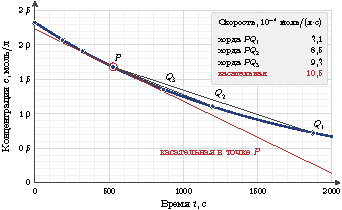
\includegraphics[width=12cm]{figs/what_is_reaction_rate/secants.pdf}
    \caption{Средние скорости разложения \ce{N2O5} на всё более коротких промежутках, начинающихся в точке $P$ ($t = \qty{526}{\ruS}$), приближаются к наклону касательной в этой точке. Наклоны хорд вычислены по данным табл.~\ref{tab:n2o5_decomposition}.}
    \label{fig:secants}
\end{figure}

Наклон касательной в точке представляет собой \term{мгновенную скорость}{instantaneous_rate}{мгновенная скорость}~--- предел, к которому стремится средняя скорость, если промежуток $\Delta t$ будет становиться всё меньше и меньше. В математике такой предел называют \emph{производной} и записывают как $\mathrm{d}c/\mathrm{d}t$. Буква d вместо $\Delta$ говорит о том, что изменения $c$ и $t$ бесконечно малы. Таким образом, мгновенная скорость по реагенту A равна
\begin{equation}
    \label{eq:instantaneous_rate}
    v(\mathrm{A}) = -\frac{\mathrm{d}c(\mathrm{A})}{\mathrm{d}t},
\end{equation}
а по продукту B будет равна $v(\mathrm{B}) = \mathrm{d}c(\mathrm{B})/\mathrm{d}t$ (без минуса).

На практике расчёт мгновенной скорости делается довольно просто. На графике проводят касательную к кривой в нужной точке, затем выбирают на ней две точки подальше друг от друга (на \emph{касательной}, а не на кривой) и делят разность концентраций на разность времён. Например, касательная на рис.~\ref{fig:secants} пересекает левую границу графика ($t = 0$) при $c \approx \qty{2,23}{\ruMole\per\ruL}$, а правую ($t = \qty{2000}{\ruS}$)~--- при $c \approx \qty{0,13}{\ruMole\per\ruL}$. Значит, в момент времени \qty{526}{\ruS}

\begin{equation*}
    v(\ce{N2O5}) \approx \frac{\num{2,23} - \num{0,13}}{2000 - 0} \approx \qty{1,05e-3}{\ruMole\per\ruL\ruS}.
\end{equation*}

Хорды, проведённые из $P$ к более \emph{ранним} точкам, дают значения скорости больше, чем в точке $P$: \qty{1,11e-3}{\ruMole\per\ruL\ruS} для промежутка \num{319}--\qty{526}{\ruS} и \qty{1,24e-3}{\ruMole\per\ruL\ruS} для промежутка \num{0}--\qty{526}{\ruS}. Таким образом, мгновенная скорость лежит между средними скоростями до и после рассматриваемой точки. При этом гораздо точнее её можно рассчитать по средней скорости на промежутке, который охватывает $P$ с обеих сторон. В данном случае для промежутка от 319 до \qty{867}{\ruS} она равна \qty{1,02e-3}{\ruMole\per\ruL\ruS}. Этим удобно пользоваться, когда касательную провести трудно (например, в задаче~\ref{prob:what_is_reaction_rate7}).

Особенно важной является мгновенная скорость в момент, когда реакция стартовала (при $t = 0$). Её называют \term{начальной скоростью}{initial_rate}{начальная скорость} реакции и обозначают $v_0$. В начале эксперимента состав реакционной смеси известен точно (мы же сами её приготовили), поэтому начальную скорость проще всего сопоставлять с концентрациями веществ. Так мы и будем поступать в следующих разделах. Для разложения \ce{N2O5} её можно найти по касательной к началу кинетической кривой на рис.~\ref{fig:kinetic_curves} (задача~\ref{prob:what_is_reaction_rate2}).

\subsection*{Скорость по веществу и скорость реакции}

Для реакций, в которых имеется несколько реагентов или продуктов, возникает вопрос: по какому веществу следить за реакцией? Для реакции~\eqref{ce:n2o5_decomposition} есть существенная разница в том, как это делать. Скорость роста концентрации \ce{N2O4} равна скорости падения концентрации \ce{N2O5}. Кислорода же за то же время образуется вдвое меньше, поскольку на каждые две разложившиеся молекулы \ce{N2O5} приходится одна образовавшаяся молекула \ce{O2}. Кислород при этом покидает раствор, так что говорить о его концентрации не имеет смысла, но скорость его образования в расчёте на литр раствора можно определить через количество вещества:

\begin{equation*}
    v(\ce{O2}) = \frac{1}{V}\,\frac{\mathrm{d}n(\ce{O2})}{\mathrm{d}t} = \frac{1}{2}\,v(\ce{N2O5}).
\end{equation*}

Скорости по разным веществам одной реакции могут различаться, но они всегда будут связаны между собой через коэффициенты в уравнении реакции. Как мы видели, когда \hyperref[sec:calculations_based_on_chemical_equations]{вели расчёты по уравнениям реакций}, количества прореагировавших и образовавшихся веществ пропорциональны их коэффициентам. Значит, и за любой промежуток времени количества всех участников меняются пропорционально коэффициентам, то есть величина $|\Delta n_i|/s_i$ для всех участников одна и та же. Поэтому, если разделить скорость по каждому веществу на его коэффициент, то для всех участников реакции получится одно и то же число. Его и называют \term{скоростью реакции}{reaction_rate}{скорость реакции}. Для реакции, в которой A~--- любой из реагентов, а B~--- любой из продуктов,

\begin{equation}
    \label{eq:reaction_rate}
    \boxed{v = -\frac{1}{s_{\mathrm{A}}}\,\frac{\mathrm{d}c(\mathrm{A})}{\mathrm{d}t} = \frac{1}{s_{\mathrm{B}}}\,\frac{\mathrm{d}c(\mathrm{B})}{\mathrm{d}t}},
\end{equation}

где $s_{\mathrm{A}}$ и $s_{\mathrm{B}}$~--- коэффициенты перед этими веществами в уравнении реакции\footnote{Формула~\eqref{eq:reaction_rate} верна, пока объём реакционной смеси не меняется, как, например, в растворе или в закрытом сосуде. В общем случае нам нужно представить эту формулу немного по-другому, где вместо изменения концентрации следует подставить изменение количества вещества, отнесённое к объёму: $v = \frac{1}{s_i V}\left|\frac{\mathrm{d}n_i}{\mathrm{d}t}\right|$. Так мы сделали с кислородом в объяснении выше.}. Для реакции разложения \ce{N2O5} по уравнению~\eqref{ce:n2o5_decomposition}

\begin{equation*}
    v = \frac{1}{2}\,v(\ce{N2O5}) = \frac{1}{2}\,v(\ce{N2O4}) = v(\ce{O2}).
\end{equation*}

Например, в момент времени, равный \qty{526}{\ruS}, \ce{N2O5} расходуется, а \ce{N2O4} образуется со скоростью \qty{1,05e-3}{\ruMole\per\ruL\ruS}, кислород образуется вдвое медленнее, со скоростью \qty{5,2e-4}{\ruMole\per\ruL\ruS}, и скорость реакции тоже равна \qty{5,2e-4}{\ruMole\per\ruL\ruS}.

При использовании скорости реакции есть нюанс, который заключается в том, что её значение зависит от того, \emph{как записано уравнение}. Если записать реакцию в виде \ce{N2O5 -> N2O4 + 1/2O2}, скорость реакции станет равной $v(\ce{N2O5})$, то есть вдвое больше, хотя в реальном мире ничего не изменилось. Но при этом скорости по веществам останутся прежними (потому что это измеряемые величины). Это аналогично тепловому эффекту \hyperref[term:thermochemical_equation]{термохимического уравнения}, который тоже удваивается при удвоении коэффициентов. Поэтому, говоря о скорости реакции, необходимо указывать и уравнение, к которому она относится.

\subsection*{Единицы скорости. Реакции на поверхности}

Скорость реакции обычно выражают в \unit{\ruMole\per\ruL\ruS}. Если процесс очень медленный, то можно использовать \unit{\ruMole\per\ruL\ruMin} или даже \unit{\ruMole\per\ruL\ruCh}. В системе СИ объём измеряют в кубических метрах, в этом случае $\qty{1}{\ruMole\per\ruL\ruS} = \qty{1000}{\ruMole\per\ruM\cubed\ruS}$.

Если реакция протекает в газовой фазе, то удобнее использовать не концентрации, а давления. Согласно уравнению состояния идеального газа~\eqref{eq:ideal_gas_law} $c = n/V = p/(RT)$, то есть при постоянной температуре концентрация газа пропорциональна его давлению (если мы рассматриваем смесь, то \emph{парциальному давлению}~--- той части общего давления, которая приходится на этот газ). Поэтому скорость газовой реакции можно выразить в единицах давления за единицу времени, например в \unit{\ruPa\per\ruS}, или перевести её при необходимости в \unit{\ruMole\per\ruM\cubed\ruS}, разделив на $RT$.

А что нам делать с реакциями, которые идут на поверхности (например, коррозия)? Назовём \term{фазой}{phase}{фаза} часть системы, одинаковую по составу и свойствам во всех своих точках и отделённую от остальных частей поверхностью раздела. Отдельной фазой будет являться раствор, кусок металла, газ над ними и т.~п. Если реакция протекает внутри одной фазы (например, в растворе или в газовой смеси), то её называют \term{гомогенной}{homogeneous_reaction}{гомогенная реакция}, а если на границе двух фаз (к примеру, металл в кислоте, горение угля, ржавление железа)~--- то \term{гетерогенной}{heterogeneous_reaction}{гетерогенная реакция}.

Гетерогенная реакция идёт только там, где фазы соприкасаются, поэтому её скорость относится не к объёму, а к площади поверхности раздела $A_{\text{пов}}$ и выражается в \unit{\ruMole\per\ruM\squared\ruS}:

\begin{equation}
    \label{eq:surface_reaction_rate}
    v = \frac{1}{s_i A_{\text{пов}}}\,\frac{|\Delta n_i|}{\Delta t}.
\end{equation}

Если мы разрежем металлическую пластинку на маленькие кусочки, то общая площадь поверхности станет больше и за секунду прореагирует больше металла, но в расчёте на квадратный метр скорость останется прежней.

Когда рассматривают реально протекающую коррозию (в инженерных расчётах), то вместо молей берут граммы, а вместо секунд~--- годы. К примеру, в городском воздухе сталь в результате коррозии теряет за год от 200 до \qty{400}{\ruG} металла с каждого квадратного метра поверхности, то есть слой толщиной \num{25}--\qty{50}{\ruUm}.

\subsection*{Как измерить скорость реакции}

Как это ни странно, не существует прибора, который показывал бы скорость реакции напрямую. На практике определение скорости заключается в измерении концентрации реагента или продукта (или величины, однозначно с ней связанной) в определённые моменты времени, а затем построении кинетической кривой и определении скорости по ней. При этом способы определения концентрации делятся на две большие группы.

\emph{Химические методы.} Из реакционной смеси через определённые промежутки времени отбирают небольшие объёмы проб и анализируют их, например титрованием или хроматографией. При этом во время измерения в пробе продолжается реакция, поэтому пробу тем или иным способом <<замораживают>>, например, резко охлаждают, сильно разбавляют или добавляют вещество, которое останавливает реакцию (например, связывают кислоту щёлочью). Это универсальный способ, впрочем, он даёт лишь отдельные точки.

\emph{Физические методы.} Также можно анализировать какое-либо свойство смеси, которое меняется в ходе реакции и связано с концентрацией веществ. Смесь при этом не трогают, а измерение чаще всего ведут непрерывно и записывают автоматически. Самые распространённые варианты таких методов приведены в табл.~\ref{tab:rate_measurement_methods}.

\begin{table}[htbp]
    \small
    \caption{Измеряемые показатели при определении скорости реакции.}
    \label{tab:rate_measurement_methods}
    \begin{tabularx}{\textwidth}{
        >{\hsize=0.85\hsize}Y
        >{\hsize=0.95\hsize}Y
        >{\hsize=1.2\hsize}Y
        }
        \hline
        \rowcolor{table_header}
        Что измеряют & Когда это возможно & Пример \\
        \hline
        Объём выделившегося газа & Выделяется газ, который легко собрать & \ce{2N2O5 -> 2N2O4 + O2 (^)} в растворе; \ce{Mg + 2HCl -> MgCl2 + H2 (^)} \\
        \hline
        Давление в закрытом сосуде & Реакция в газовой фазе, при которой меняется число молекул газа & \ce{2O3 -> 3O2}: из двух молекул газа получаются три \\
        \hline
        Массу реакционной смеси & Газ уходит из открытого сосуда & \ce{CaCO3 + 2HCl -> CaCl2 + H2O + CO2 (^)} \\
        \hline
        Окраску (поглощение света) & Хотя бы один из участников окрашен & Раствор перманганата калия обесцвечивается щавелевой кислотой \\
        \hline
        Электропроводность раствора & Меняется число ионов в растворе & \ce{(CH3)3CCl + H2O -> (CH3)3COH + HCl}: в растворе появляются ионы \ce{H+} и \ce{Cl-} \\
        \hline
        Угол поворота плоскости поляризации света & Участвуют оптически активные вещества & Гидролиз сахарозы \\
        \hline
    \end{tabularx}
\end{table}

Например, чем больше в растворе окрашенного вещества, тем сильнее он поглощает свет. Это можно измерить при помощи фотоколориметра, который показывает, какая доля исходного света прошла через раствор (не поглотилась). Также растворы некоторых веществ (например, сахаров) поворачивают плоскость поляризации проходящего через них света, и угол поворота пропорционален концентрации. Угол поворота измеряют при помощи прибора, называющегося поляриметром. Именно так впервые в истории удалось измерить скорость химической реакции (немецкий физик Людвиг Вильгельми в 1850~году измерил скорость гидролиза сахарозы в присутствии кислоты).

Данные, приведённые в табл.~\ref{tab:n2o5_decomposition}, получены расчётным путём по объёму выделившегося газа. Эйринг и Даниэлс собирали выделявшийся кислород в газовую бюретку и измеряли его объём, а концентрации \ce{N2O5} вычислены из этого объёма по уравнению реакции\footnote{Колба вместимостью \qty{5}{\ruMl} с раствором находилась в термостате, где температура колебалась не больше чем на \qty{0,01}{\degreeCelsius}. Колбу встряхивали 360~раз в минуту. Это нужно было для того, чтобы кислород не оставался в растворе. Выделяющийся газ проходил через стекловату, смоченную концентрированной серной кислотой, которая поглощала диоксид азота, тоже присутствовавший в газовой смеси.}. Упрощённая схема этого эксперимента и его результаты показаны на рис.~\ref{fig:gas_syringe}.

\begin{figure}[htbp]
    \centering
    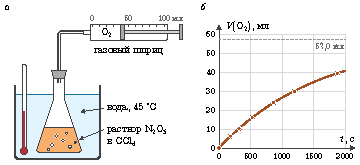
\includegraphics[width=12cm]{figs/what_is_reaction_rate/gas_syringe.pdf}
    \caption{Эксперимент по измерению скорости разложения \ce{N2O5} через объём выделившегося кислорода: \emph{а}~--- упрощённая схема опыта: колба с раствором стоит в термостате при \qty{45}{\degreeCelsius}, кислород собирается в газовый шприц; \emph{б}~--- объём выделившегося кислорода для \qty{2,00}{\ruMl} раствора из табл.~\ref{tab:n2o5_decomposition} (в пересчёте на \qty{25}{\degreeCelsius} и \qty{101,3}{\ruKPa}). Пунктир~--- объём после полного разложения \ce{N2O5}.}
    \label{fig:gas_syringe}
\end{figure}

\begin{example}{}{what_is_reaction_rate2}
    \begin{condition}
        В колбу налили \qty{2,00}{\ruMl} раствора \ce{N2O5} в \ce{CCl4} из табл.~\ref{tab:n2o5_decomposition}. За первые \qty{184}{\ruS} в шприце собралось \qty{6,25}{\ruMl} кислорода (объём приведён к \qty{25}{\degreeCelsius} и давлению \qty{101,3}{\ruKPa}). Какова концентрация \ce{N2O5} в этот момент? Какой объём кислорода соберётся, когда весь \ce{N2O5} разложится?
    \end{condition}

    \medskip

    \textit{Решение.} Количество кислорода найдём из уравнения состояния идеального газа~\eqref{eq:ideal_gas_law}:

    \begin{equation*}
        n(\ce{O2}) = \frac{pV}{RT} = \frac{\num{101300} \cdot \num{6,25e-6}}{\num{8,314} \cdot 298} = \qty{2,56e-4}{\ruMole}.
    \end{equation*}

    По уравнению~\eqref{ce:n2o5_decomposition} две молекулы \ce{N2O5} приводят к образованию одной молекулы кислорода, поэтому к этому моменту разложилось $2n(\ce{O2}) = \qty{5,12e-4}{\ruMole}$ \ce{N2O5}, и его концентрация уменьшилась на

    \begin{equation*}
        \Delta c = \frac{\qty{5,12e-4}{\ruMole}}{\qty{2,00e-3}{\ruL}} = \qty{0,256}{\ruMole\per\ruL}.
    \end{equation*}

    К моменту времени \qty{184}{\ruS} концентрация \ce{N2O5} стала равна $\num{2,33} - \num{0,256} \approx \qty{2,07}{\ruMole\per\ruL}$ (это значение и стоит в табл.~\ref{tab:n2o5_decomposition})\footnote{Вместе с кислородом из колбы уходят ещё и пары растворителя. Но мы для простоты считаем газ в шприце чистым кислородом.}.

    К моменту окончания реакции кислорода выделится вдвое меньше, чем изначально было \ce{N2O5}:
    \begin{equation*}
        n(\ce{O2}) = \frac{1}{2} \cdot \qty{2,33}{\ruMole\per\ruL} \cdot \qty{2,00e-3}{\ruL} = \qty{2,33e-3}{\ruMole},
    \end{equation*}
    то есть
    \begin{equation*}
        V = \frac{nRT}{p} = \frac{\num{2,33e-3} \cdot \num{8,314} \cdot 298}{\num{101300}} = \qty{5,70e-5}{\ruM\cubed} = \qty{57,0}{\ruMl}.
    \end{equation*}

    Этот объём показан на рис.~\ref{fig:gas_syringe} пунктиром.
\end{example}

Однако для очень быстрых реакций такие способы измерения скорости непригодны, потому что реакция закончится раньше, чем мы успеем смешать растворы. В этом случае реакцию инициируют импульсом света или резким нагревом, а затем следят за ней оптическими методами. За исследования таких быстропротекающих реакций Манфред Эйген, Рональд Норриш и Джордж Портер получили Нобелевскую премию по химии 1967~года. Позже с помощью лазерных импульсов длительностью в десятки фемтосекунд (фемтосекунда~--- это \qty{e-15}{\ruS}) удалось даже наблюдать момент, когда рвутся и образуются химические связи. Эта работа Ахмеда Зевейла была удостоена Нобелевской премии 1999~года.

\subsection*{Некоторые подводные камни}

Вам нужно чётко понимать, какую информацию несёт в себе скорость химической реакции, а какую не несёт.

Во-первых, скорость реакции ничего не говорит о том, чем закончится реакция. Для описания того, \emph{сколько} в итоге получилось продукта, используются \hyperref[term:yield]{выход реакции} и полнота превращения. Например, быстро протекающая реакция может дать низкий выход продукта, если параллельно с ней будут идти побочные реакции. Напротив, медленная реакция рано или поздно может пройти до конца. В этой главе мы пока будем считать, что реакции идут только в одну сторону, до полного расходования одного из реагентов.

Во-вторых, скорость реакции не определяется энергией Гиббса. Знак $\Delta G$ говорит, \emph{может ли} реакция идти, но не говорит, \emph{как быстро} она будет протекать. Реакция может быть термодинамически очень выгодной, но при этом идти невероятно медленно (например, превращение алмаза в графит из задачи~\ref{prob:gibbs_energy7} или взаимодействие водорода с кислородом при комнатной температуре). И наоборот, реакция с небольшим энергетическим выигрышем может идти мгновенно (задача~\ref{prob:what_is_reaction_rate5}). Термодинамика указывает только, в какую сторону будет идти реакция, а кинетика~--- как быстро и каким путём.

\begin{termlist}
    \hyperref[term:chemical_kinetics]{Химическая кинетика},
    \hyperref[term:kinetic_curve]{кинетическая кривая},
    \hyperref[term:average_rate]{средняя скорость},
    \hyperref[term:rate_by_substance]{скорость по веществу},
    \hyperref[term:instantaneous_rate]{мгновенная скорость},
    \hyperref[term:initial_rate]{начальная скорость},
    \hyperref[term:reaction_rate]{скорость реакции},
    \hyperref[term:phase]{фаза},
    \hyperref[term:homogeneous_reaction]{гомогенная реакция},
    \hyperref[term:heterogeneous_reaction]{гетерогенная реакция}.
\end{termlist}

\begin{problem}{}{what_is_reaction_rate1}
    По данным табл.~\ref{tab:n2o5_decomposition} вычислите средние скорости разложения \ce{N2O5} на каждом из шести промежутков между соседними измерениями. Как меняется скорость со временем? Сколько \ce{N2O5} разложилось бы за первые \qty{184}{\ruS}, если бы реакция в течение всего времени шла со средней скоростью за всё время наблюдения, найденной в примере~\ref{ex:what_is_reaction_rate1}? Проведите сравнение с тем, что было на самом деле.
    \begin{sol}{\ref{prob:what_is_reaction_rate1}}
        По формуле~\eqref{eq:average_rate} получаем:

        \begin{center}
            \small
            \begin{tabular}{cccc}
                \hline
                \rowcolor{table_header}
                Промежуток, с & $\Delta c$, \unit{\ruMole\per\ruL} & $\Delta t$, с & $\overline{v}$, \unit{\ruMole\per\ruL\ruS} \\
                \hline
                0--184 & \num{0,26} & 184 & \num{1,41e-3} \\
                184--319 & \num{0,16} & 135 & \num{1,19e-3} \\
                319--526 & \num{0,23} & 207 & \num{1,11e-3} \\
                526--867 & \num{0,33} & 341 & \num{9,7e-4} \\
                867--1198 & \num{0,24} & 331 & \num{7,3e-4} \\
                1198--1877 & \num{0,39} & 679 & \num{5,7e-4} \\
                \hline
            \end{tabular}
        \end{center}

        Скорость реакции монотонно уменьшается. К концу опыта она упала почти в два с половиной раза. Если бы реакция всё время шла со средней скоростью \qty{8,58e-4}{\ruMole\per\ruL\ruS}, за первые \qty{184}{\ruS} разложилось бы $\num{8,58e-4} \cdot 184 \approx \qty{0,16}{\ruMole\per\ruL}$ \ce{N2O5}, а на самом деле разложилось \qty{0,26}{\ruMole\per\ruL}, в \num{1,6}~раза больше.
    \end{sol}
\end{problem}

\begin{problem}{}{what_is_reaction_rate2}
    На рис.~\ref{fig:kinetic_curves} проведены касательные к кинетическим кривым в начальный момент времени и в момент $t = \qty{1700}{\ruS}$.
    \begin{enumerate}[label=\arabic*)]
        \item По касательным найдите начальную скорость разложения \ce{N2O5} и скорость в момент $t = \qty{1700}{\ruS}$.
        \item Чему равны в эти моменты скорость образования \ce{N2O4}, скорость образования кислорода (в расчёте на литр раствора) и скорость реакции~\eqref{ce:n2o5_decomposition}?
        \item Во сколько раз уменьшилась скорость разложения \ce{N2O5} за \qty{1700}{\ruS}? Во сколько раз за то же время уменьшилась концентрация \ce{N2O5} (её значение в момент $t = \qty{1700}{\ruS}$ найдите по графику)?
    \end{enumerate}
    \begin{sol}{\ref{prob:what_is_reaction_rate2}}
        1)~Начальная касательная проходит через точки (0;~\num{2,33}) и (500;~\num{1,60}), поэтому

        \begin{equation*}
            v_0(\ce{N2O5}) = \frac{\num{2,33} - \num{1,60}}{500} = \qty{1,46e-3}{\ruMole\per\ruL\ruS}.
        \end{equation*}

        Касательная в момент $t = \qty{1700}{\ruS}$ проходит через точки (1200;~\num{1,06}) и (2200;~\num{0,55}), и

        \begin{equation*}
            v(\ce{N2O5}) = \frac{\num{1,06} - \num{0,55}}{1000} = \qty{5,1e-4}{\ruMole\per\ruL\ruS}.
        \end{equation*}

        Ваши значения могут немного отличаться~--- это не страшно: всё зависит от того, насколько точно вы считываете координаты с графика.

        2)~Касательные к кривой \ce{N2O4} зеркальны касательным к кривой \ce{N2O5}, поэтому \ce{N2O4} образуется с той же скоростью \num{1,46e-3} и \qty{5,1e-4}{\ruMole\per\ruL\ruS}. Кислорода по уравнению~\eqref{ce:n2o5_decomposition} образуется вдвое меньше, около \num{7,3e-4} и \qty{2,5e-4}{\ruMole\per\ruL\ruS}. Скорость реакции по формуле~\eqref{eq:reaction_rate} равна $v = \frac{1}{2}v(\ce{N2O5})$, то есть тоже \num{7,3e-4} и \qty{2,5e-4}{\ruMole\per\ruL\ruS}.

        3)~Скорость уменьшилась в $\num{1,46e-3}/\num{5,1e-4} \approx \num{2,9}$~раза. Концентрация \ce{N2O5} в момент $t = \qty{1700}{\ruS}$ по графику около \qty{0,81}{\ruMole\per\ruL}, то есть она уменьшилась в $\num{2,33}/\num{0,81} \approx \num{2,9}$~раза~--- так же, как и скорость. Это логично, поскольку скорость этой реакции пропорциональна концентрации \ce{N2O5}. Подробнее об этом~--- в следующем разделе.
    \end{sol}
\end{problem}

\begin{problem}{}{what_is_reaction_rate3}
    Реакцию пероксида водорода с иодидом калия в кислой среде
    \reaction*{H2O2 + 2KI + H2SO4 -> I2 + K2SO4 + 2H2O}
    одной из первых изучили количественно (ещё в 1860-х годах). В некоторый момент времени иод образуется со скоростью \qty{2,0e-5}{\ruMole\per\ruL\ruS}.
    \begin{enumerate}[label=\arabic*)]
        \item С какой скоростью в этот момент расходуются пероксид водорода, иодид калия и серная кислота? Чему равна скорость реакции?
        \item Выразите скорость расходования иодида калия в \unit{\ruMole\per\ruL\ruMin} и в \unit{\ruMole\per\ruM\cubed\ruS}.
        \item Как изменятся найденные величины, если записать уравнение с коэффициентами, вдвое меньшими?
    \end{enumerate}
    \begin{sol}{\ref{prob:what_is_reaction_rate3}}
        1)~По формуле~\eqref{eq:reaction_rate} скорость реакции равна скорости образования иода, делённой на его коэффициент:
        \begin{equation*}
            v = \frac{v(\ce{I2})}{1} = \qty{2,0e-5}{\ruMole\per\ruL\ruS}.
        \end{equation*}

        Отсюда
        \begin{equation*}
            v(\ce{H2O2}) = v(\ce{H2SO4}) = v = \qty{2,0e-5}{\ruMole\per\ruL\ruS},
        \end{equation*}
        \begin{equation*}
            v(\ce{KI}) = 2v = \qty{4,0e-5}{\ruMole\per\ruL\ruS}.
        \end{equation*}

        2)~Минута в 60 раз длиннее секунды, а кубический метр в 1000 раз больше литра:
        \begin{equation*}
            \qty{4,0e-5}{\ruMole\per\ruL\ruS} \cdot \qty{60}{\ruS\per\ruMin} = \qty{2,4e-3}{\ruMole\per\ruL\ruMin},
        \end{equation*}
        \begin{equation*}
            \qty{4,0e-5}{\ruMole\per\ruL\ruS} \cdot \qty{1000}{\ruL\per\ruM\cubed} = \qty{4,0e-2}{\ruMole\per\ruM\cubed\ruS}.
        \end{equation*}

        3)~Скорости по веществам~--- это измеряемые величины, поэтому от записи уравнения они не зависят. А вот скорость реакции вырастет вдвое:
        \begin{equation*}
            v = \frac{v(\ce{I2})}{1/2} = \qty{4,0e-5}{\ruMole\per\ruL\ruS}.
        \end{equation*}
    \end{sol}
\end{problem}

\begin{problem}{}{what_is_reaction_rate4}
    Каким способом вы бы предпочли следить за ходом каждой из указанных реакций? Объясните свой выбор.
    \begin{enumerate}[label=\arabic*)]
        \item Кусочки мрамора растворяются в соляной кислоте: \ce{CaCO3 + 2HCl -> CaCl2 + H2O + CO2 (^)}.
        \item Цинковая пластинка опущена в раствор сульфата меди (II): \ce{Zn + CuSO4 -> ZnSO4 + Cu}.
        \item При \qty{500}{\degreeCelsius} циклопропан превращается в пропен \ce{CH2=CH-CH3}; оба вещества~--- бесцветные газы.
        \item Озон разлагается в закрытом сосуде: \ce{2O3 -> 3O2}.
        \item Этилацетат гидролизуется раствором гидроксида натрия: \ce{CH3COOC2H5 + NaOH -> CH3COONa + C2H5OH}.
    \end{enumerate}
    \begin{sol}{\ref{prob:what_is_reaction_rate4}}
        1)~Углекислый газ уходит из открытой колбы, поэтому удобно поставить колбу на весы и следить за уменьшением массы (горлышко закрывают ватой, чтобы вместе с газом не вылетали брызги кислоты). Можно также собирать газ в шприц.

        2)~Раствор сульфата меди (II) голубой, а сульфат цинка бесцветен, поэтому окраска бледнеет по мере протекания реакции, и за ней можно следить фотоколориметром.

        3)~Здесь из одной молекулы газа получается одна молекула газа, поэтому давление в закрытом сосуде не меняется, при этом оба газа бесцветны. Что ж, остаётся только отбирать пробы и анализировать их состав.

        4)~Из двух молекул газа получаются три, поэтому давление в закрытом сосуде растёт (после окончания реакции оно вырастет в полтора раза). Также можно использовать способность озона поглощать ультрафиолетовое излучение.

        5)~Щёлочь расходуется, поэтому можно отбирать пробы, <<замораживать>> их избытком кислоты известной концентрации, а затем оттитровывать остаток кислоты. Также можно следить за электропроводностью, используя тот факт, что гидроксид-ионы проводят ток гораздо лучше ацетат-ионов, которые их заменяют, из-за чего электропроводность раствора будет падать по мере протекания реакции.
    \end{sol}
\end{problem}

\begin{problem}{}{what_is_reaction_rate5}
    Профессор Недоумелкин сравнивает реакции: образование воды из водорода и кислорода ($\Delta G^{\circ} = \qty{-237}{\ruKJ}$ на моль воды) и нейтрализацию соляной кислоты гидроксидом натрия ($\Delta G^{\circ} \approx \qty{-80}{\ruKJ}$ на моль воды). <<Первая реакция втрое выгоднее, значит, она и идёт втрое быстрее>>,~--- заключает он. Что вы ему ответите?
    \begin{sol}{\ref{prob:what_is_reaction_rate5}}
        Энергия Гиббса отвечает на вопрос, может ли реакция идти, но ничего не говорит о её скорости. На деле смесь водорода с кислородом при комнатной температуре может годами храниться без заметных изменений, пока её не подожгут, а нейтрализация в растворе проходит мгновенно. Ионы \ce{H+} и \ce{OH-} соединяются практически при каждой встрече~--- это одна из самых быстрых реакций в растворе. На практике её скорость ограничивает скорость перемешивания растворов.

        Можно рассуждать и по-другому. Если поджечь смесь водорода с кислородом, то скорость реакции вырастет на много порядков, хотя $\Delta G$ останется прежним. Значит, скорость определяется чем-то другим. Чем именно, мы объясним в следующих разделах.
    \end{sol}
\end{problem}

\begin{problem}{}{what_is_reaction_rate6}
    $\bigstar$ Ленту магния массой \qty{0,048}{\ruG} опустили в \qty{50,0}{\ruMl} соляной кислоты с концентрацией \qty{1,00}{\ruMole\per\ruL}, а выделяющийся водород собирали в газовый шприц. За первые \qty{30}{\ruS} набралось \qty{24,0}{\ruMl} газа при \qty{20}{\degreeCelsius} и \qty{101,3}{\ruKPa}.
    \begin{enumerate}[label=\arabic*)]
        \item Какое количество водорода выделилось и какая доля магния успела прореагировать?
        \item Найдите среднюю скорость расходования \ce{HCl} и среднюю скорость реакции за эти \qty{30}{\ruS} в \unit{\ruMole\per\ruL\ruS}. Как при этом изменилась концентрация кислоты?
        \item Реакция идёт на поверхности металла, площадь которой в начале опыта около \qty{3,0}{\ruCm\squared}. Найдите среднюю скорость реакции в \unit{\ruMole\per\ruM\squared\ruS}.
        \item Во сколько раз магний растворяется в кислоте быстрее, чем ржавеет сталь в городском воздухе (\num{200}--\qty{400}{\ruG} железа с квадратного метра в год)?
    \end{enumerate}
    \begin{sol}{\ref{prob:what_is_reaction_rate6}}
        1)~Из уравнения состояния идеального газа
        \begin{equation*}
            n(\ce{H2}) = \frac{pV}{RT} = \frac{\num{101300} \cdot \num{24,0e-6}}{\num{8,314} \cdot 293} = \num{9,98e-4} \approx \qty{1,00e-3}{\ruMole}.
        \end{equation*}

        Магния было $\num{0,048}/\num{24,31} = \qty{1,97e-3}{\ruMole}$. По уравнению \ce{Mg + 2HCl -> MgCl2 + H2 (^)} на каждый моль водорода расходуется моль магния, значит, прореагировала примерно половина магния.

        2)~Кислоты израсходовано вдвое больше, чем выделилось водорода: $\Delta n(\ce{HCl}) = \qty{2,00e-3}{\ruMole}$, поэтому
        \begin{equation*}
            \Delta c(\ce{HCl}) = \frac{\qty{2,00e-3}{\ruMole}}{\qty{0,0500}{\ruL}} = \qty{0,0400}{\ruMole\per\ruL},
        \end{equation*}
        а средняя скорость расходования \ce{HCl} за \qty{30}{\ruS}
        \begin{equation*}
            \overline{v}(\ce{HCl}) = \frac{\qty{0,0400}{\ruMole\per\ruL}}{\qty{30}{\ruS}} = \qty{1,33e-3}{\ruMole\per\ruL\ruS}.
        \end{equation*}

        Скорость реакции по формуле~\eqref{eq:reaction_rate} вдвое меньше: \qty{6,7e-4}{\ruMole\per\ruL\ruS}. Концентрация кислоты уменьшилась всего с \num{1,00} до \qty{0,96}{\ruMole\per\ruL}, потому что кислота взята в большом избытке.

        3)~По формуле~\eqref{eq:surface_reaction_rate}
        \begin{equation*}
            v = \frac{\num{1,00e-3}}{\num{3,0e-4} \cdot 30} \approx \qty{0,11}{\ruMole\per\ruM\squared\ruS}.
        \end{equation*}

        4)~Сталь теряет \num{200}--\qty{400}{\ruG}, то есть \num{3,6}--\qty{7,2}{\ruMole} железа с квадратного метра за год, а в году \qty{3,16e7}{\ruS}. Это \num{1,1e-7}--\qty{2,3e-7}{\ruMole\per\ruM\squared\ruS}. Отношение скоростей
        \begin{equation*}
            \frac{\num{0,11}}{\num{2,3e-7}} \approx \num{5e5} \quad\text{и}\quad \frac{\num{0,11}}{\num{1,1e-7}} \approx \num{1e6},
        \end{equation*}
        то есть магний в кислоте растворяется в полмиллиона~--- миллион раз быстрее.
    \end{sol}
\end{problem}

\begin{problem}{}{what_is_reaction_rate7}
    $\bigstar$ Если трудно провести касательную к кинетической кривой, мгновенную скорость оценивают через среднюю скорость на коротком промежутке (точка при этом должна лежать на его середине).
    \begin{enumerate}[label=\arabic*)]
        \item Используя результаты задачи~\ref{prob:what_is_reaction_rate1}, постройте график зависимости скорости разложения \ce{N2O5} от времени, откладывая каждую среднюю скорость в середине своего промежутка.
        \item Для каждого промежутка найдите среднюю концентрацию \ce{N2O5} (полусумму значений на его концах) и постройте график зависимости скорости от концентрации. Что вы замечаете?
        \item С какой скоростью разлагался бы \ce{N2O5} в растворе с концентрацией \qty{1,00}{\ruMole\per\ruL} при той же температуре?
    \end{enumerate}
    \begin{sol}{\ref{prob:what_is_reaction_rate7}}
        1)~Середины промежутков приходятся на 92, 252, 423, 697, 1033 и \qty{1538}{\ruS}, а скорости (в единицах \qty{e-4}{\ruMole\per\ruL\ruS}) равны \num{14,1}; \num{11,9}; \num{11,1}; \num{9,7}; \num{7,3} и \num{5,7}. Точки ложатся на плавную убывающую кривую, похожую по форме на саму кинетическую кривую \ce{N2O5}.

        2)~Средние концентрации равны \num{2,20}; \num{1,99}; \num{1,80}; \num{1,52}; \num{1,23} и \qty{0,92}{\ruMole\per\ruL}. На графике <<скорость~--- концентрация>> точки ложатся на прямую, проходящую через начало координат: отношение скорости к концентрации почти одно и то же, от \num{5,9e-4} до \qty{6,4e-4}{\ruS\tothe{-1}}, в среднем \qty{6,2e-4}{\ruS\tothe{-1}}. Значит, скорость разложения \ce{N2O5} пропорциональна его концентрации. Именно поэтому в задаче~\ref{prob:what_is_reaction_rate2} скорость и концентрация уменьшились в одно и то же число раз.

        3)~Скорость пропорциональна концентрации, поэтому
        \begin{equation*}
            v = \qty{6,2e-4}{\ruS\tothe{-1}} \cdot \qty{1,00}{\ruMole\per\ruL} = \qty{6,2e-4}{\ruMole\per\ruL\ruS}.
        \end{equation*}

        Такие зависимости скорости от концентрации мы будем изучать в следующем разделе. Настоящий опыт дал бы чуть меньшее значение: Эйринг и Даниэлс заметили, что в растворах с меньшей начальной концентрацией отношение скорости к концентрации немного меньше. В опыте, начатом с \qty{1,40}{\ruMole\per\ruL}, оно было в среднем \qty{6,0e-4}{\ruS\tothe{-1}}.
    \end{sol}
\end{problem}

\clearpage

\section{Что влияет на скорость реакции}

Теперь вы понимаете, что такое скорость реакции. В этом разделе мы рассмотрим, как мы можем ею управлять (в определённых пределах). Управление скоростями химических реакций~--- это одна из основных инженерных задач химии как практической науки, и в вашей карьере химика вы обязательно встретитесь с ситуациями, когда вам будет нужно ускорить полезные реакции и замедлить нежелательные.

Для начала рассмотрим теоретические подходы к управлению скоростью и затем покажем, как эти подходы работают на конкретных примерах.

\subsection*{Модель столкновений}

Очевидно, что частицы должны встретиться для того, чтобы прореагировать. Одна молекула не сможет вступить в реакцию с другой молекулой, если та будет находиться на другом конце сосуда, для этого должен произойти контакт частиц (столкновение). Представление о том, что химическая реакция происходит при столкновениях частиц реагентов, называют \term{моделью столкновений}{collision_model}{модель столкновений}.

Уже из этого определения становится понятно, что чем чаще будут сталкиваться частицы, тем быстрее будет идти реакция. Однако не каждое столкновение приводит к химической реакции~--- частицы могут разлететься, не прореагировав. В ходе реакции происходит разрыв одних \hyperref[sec:introduction_to_chemical_bonding]{химических связей} и образование других, и для этого должны выполняться два условия (рис.~\ref{fig:collision_outcomes}).

\begin{itemize}
    \item \emph{Энергия.} Частицы должны столкнуться достаточно сильно (обладать достаточной энергией). Если энергия сталкивающихся частиц будет слишком мала, её не хватит на разрыв исходных связей, и молекулы разлетятся.
    \item \emph{Ориентация.} Частицы должны не просто столкнуться, а сделать это <<нужными местами>>. Например, в реакции \ce{NO + O3 -> NO2 + O2} молекула оксида азота (II) образует новую связь \ce{N\bond{1}O} не с центральным, а с одним из крайних атомов молекулы озона. Для этого она должна подлететь к такому атому кислорода именно атомом азота.
\end{itemize}

\begin{figure}[htbp]
    \centering
    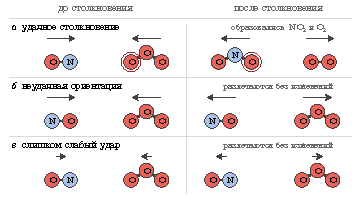
\includegraphics[width=12cm]{figs/what_affects_reaction_rate/collision_outcomes.pdf}
    \caption{Варианты столкновения молекул \ce{NO} и \ce{O3}: \emph{а}~--- молекула \ce{NO} с достаточной энергией сталкивается атомом азота с крайним атомом кислорода, реакция происходит; \emph{б}~--- молекула \ce{NO} сталкивается с озоном своим кислородным концом, молекулы разлетаются без протекания реакции; \emph{в}~--- правильная ориентация для протекания реакции, но столкновение слишком слабое, реакции нет. Длина стрелок соответствует скорости движения молекул. Обведён атом кислорода, который переходит от озона к \ce{NO}.}
    \label{fig:collision_outcomes}
\end{figure}

Столкновения, которые приводят к реакции, называют \term{эффективными}{effective_collision}{эффективное столкновение}. Таким образом, скорость реакции между частицами A и B определяется двумя множителями:
\begin{equation}
    \label{eq:collision_model}
    \boxed{\text{Скорость} \varpropto \text{Частота столкновений} \cdot \text{Доля эффективных столкновений}},
\end{equation}
где частота столкновений~--- это число столкновений частиц A с частицами B в единице объёма за единицу времени. Теперь давайте рассмотрим, какие условия влияют на первый множитель, а какие~--- на второй. Но для начала проведём пять экспериментов.

\subsection*{Пять опытов}

№~1. Мы бросаем по одинаковой грануле цинка в две пробирки, в которых находятся разбавленная и концентрированная соляная кислота. В обеих пробирках начинает протекать реакция
\reaction*{Zn + 2HCl -> ZnCl2 + H2 (^) {,}}
но в концентрированной кислоте пузырьки водорода образуются заметно чаще.

№~2. Смешаем раствор тиосульфата натрия с соляной кислотой. При этом будет протекать реакция
\reaction[ce:thiosulfate_and_acid]{Na2S2O3 + 2HCl -> 2NaCl + S (v) + SO2 (^) + H2O{.}}
Сера при этом выпадает из раствора в виде мельчайших частиц, и изначально прозрачный раствор постепенно мутнеет. Если поставить стакан с реагирующей смесью на лист бумаги с нарисованным крестиком и смотреть сквозь раствор на крестик сверху, то можно определить время, через которое крестик перестанет быть виден (рис.~\ref{fig:thiosulfate_clock},~\emph{а}). Чем быстрее идёт реакция, тем раньше в растворе будет накоплено столько серы, чтобы крестик исчез.

Теперь возьмём пять одинаковых стаканов, нальём в них 50, 40, 30, 20 и \qty{10}{\ruMl} раствора тиосульфата и дольём в стаканы воду до метки \qty{50}{\ruMl}. При этом в самом концентрированном растворе окажется в пять раз больше тиосульфата, чем в самом разбавленном. Если теперь мы добавим в каждый стакан по \qty{5}{\ruMl} соляной кислоты, то в самом концентрированном растворе крестик скроется через \qty{22,5}{\ruS}, а в самом разбавленном~--- только через \qty{159}{\ruS}\footnote{Это данные демонстрационного опыта из методической разработки Flinn Scientific <<Rate of Reaction of Sodium Thiosulfate and Hydrochloric Acid>> (Publication No.~91860, 2017). Концентрация исходного раствора тиосульфата натрия равна \qty{0,15}{\ruMolar}, соляной кислоты~--- \qty{2}{\ruMolar}.} (рис.~\ref{fig:thiosulfate_clock},~\emph{б}).

\begin{figure}[htbp]
    \centering
    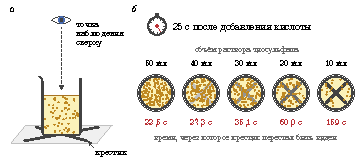
\includegraphics[width=12cm]{figs/what_affects_reaction_rate/thiosulfate_clock.pdf}
    \caption{Опыт с тиосульфатом натрия: \emph{а}~--- стакан стоит на листе бумаги с крестиком, за крестиком наблюдают сверху; \emph{б}~--- пять стаканов через \qty{25}{\ruS} после добавления кислоты, вид сверху. Над стаканами указан объём раствора тиосульфата (вода долита до \qty{50}{\ruMl}), под ними~--- время, через которое крестик скрылся полностью.}
    \label{fig:thiosulfate_clock}
\end{figure}

№~3. Внесём в пламя газовой горелки железный гвоздь, а затем комок стальной ваты (спутанной стальной проволоки толщиной в несколько сотых миллиметра). Гвоздь только раскалится. Стальная вата же загорится с рассыпанием искр и продолжит гореть, если мы вытащим её из пламени.

№~4. Подожжём деревянную лучинку (тонкую деревянную палочку), дадим ей немного погореть и задуем пламя. Лучинка продолжит тлеть. Теперь внесём её в сосуд с чистым кислородом, при этом она снова ярко вспыхнет.

№~5. Повторим второй опыт, но предварительно подогреем растворы на 10--20 градусов. При этом крестик исчезнет заметно быстрее, чем при комнатной температуре.

Обратите внимание, что в каждом нашем эксперименте реагирующие вещества оставались одними и теми же, но менялись \emph{условия проведения} реакции: концентрация раствора (в первом и втором опытах), форма, в которой взято железо (в третьем), содержание кислорода в газе (в четвёртом) и температура (в пятом).

\subsection*{Концентрация}

Чем больше частиц в единице объёма, тем чаще они сталкиваются. Допустим, каждая частица A может столкнуться с каждой частицей B, поэтому число возможных пар A--B равно произведению числа частиц A на число частиц B (рис.~\ref{fig:collision_pairs}). Если в одном и том же объёме увеличить число частиц A вдвое, то каждая частица B будет встречать частицы A в два раза чаще, и частота столкновений удвоится. Если удвоить также число частиц B, то частота столкновений вырастет вчетверо. Другими словами, частота столкновений частиц A с частицами B пропорциональна \emph{произведению их концентраций} $c(\mathrm{A}) \cdot c(\mathrm{B})$.

\begin{figure}[htbp]
    \centering
    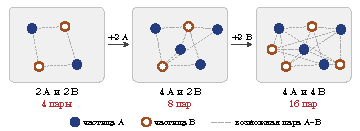
\includegraphics[width=12cm]{figs/what_affects_reaction_rate/collision_pairs.pdf}
    \caption{Возможные пары частиц A и B (соединены пунктиром) при  увеличении их количества в одном и том же объёме.}
    \label{fig:collision_pairs}
\end{figure}

Поэтому \emph{при увеличении концентрации реагентов реакция ускоряется}. Как мы видели из экспериментов, в более концентрированной кислоте цинк растворяется быстрее, а крестик скрывается раньше в более концентрированном растворе тиосульфата натрия.

Впрочем, не думайте, что скорость \emph{любой} реакции пропорциональна концентрациям реагентов. Например, давайте вернёмся к разложению этанола в крови, описанному в предыдущем разделе. Пока этанола в крови много, скорость реакции почти не зависит от его концентрации, поскольку существует ограниченное количество молекул фермента, все из которых <<работают>> в данный момент. А вот скорость разложения \ce{N2O5} (как показано в задаче~\ref{prob:what_is_reaction_rate7}) действительно пропорциональна концентрации \ce{N2O5}. Как именно скорость реакции зависит от концентрации, можно установить только по результатам измерений, и в следующем разделе мы обсудим, как это следует делать.

Второй нюанс связан с веществами-участниками реакции, концентрация которых либо не имеет смысла, либо практически не меняется. Например, гранула цинка не распределена по раствору, а её атомы встречаются с кислотой только на поверхности контакта гранулы с кислотой. Если положить в кислоту вторую такую же гранулу, водород будет выделяться вдвое быстрее, но вовсе не потому, что выросла <<концентрация цинка>>, а потому, что вдвое увеличилась поверхность металла. Не имеет также смысла что-либо говорить о концентрации растворителя. Например, в литре любого \emph{разбавленного} водного раствора содержится около \num{55}~моль воды, и это количество почти не меняется в ходе протекания реакции, даже если вода в ней участвует.

Для газов роль концентрации играет давление. Как мы показали в предыдущем разделе, концентрацию газа можно выразить как $c = p/(RT)$, то есть при постоянной температуре концентрация газа пропорциональна его парциальному давлению. Если мы сожмём смесь газов вдвое, концентрации всех газов в смеси удвоятся, а частота столкновений частиц A и B вырастет вчетверо. Мы наблюдаем это в эксперименте №~4. В нём мы фактически увеличиваем концентрацию кислорода почти в пять раз, заменив воздух (в нём содержание кислорода \qty{21}{\percent} по объёму) чистым кислородом при том же давлении.

\begin{example}{}{what_affects_reaction_rate1}
    \begin{condition}
        В закрытом сосуде при постоянной температуре находится смесь оксида азота (II) и озона, которые реагируют согласно уравнению \ce{NO + O3 -> NO2 + O2}. Во сколько раз изменится частота столкновений молекул \ce{NO} с молекулами \ce{O3}, если: а)~вдвое уменьшить объём сосуда при сохранении количества газов; б)~добавить в сосуд столько аргона, что общее давление вырастет вдвое; в)~выпустить из сосуда половину смеси?
    \end{condition}

    \medskip

    \textit{Решение.} Частота столкновений пропорциональна произведению концентраций $c(\ce{NO}) \cdot c(\ce{O3})$, а концентрация каждого газа пропорциональна его парциальному давлению.

    \medskip

    а)~Концентрации обоих газов удвоятся, следовательно, частота столкновений вырастет в $2 \cdot 2 = 4$~раза.

    \medskip

    б)~Аргон с \ce{NO} и \ce{O3} не реагирует. При этом количества \ce{NO} и \ce{O3} и объём сосуда не изменились, значит, не изменились и их концентрации (парциальные давления). Поэтому частота столкновений молекул \ce{NO} с молекулами \ce{O3} останется прежней, хотя общее давление выросло вдвое. Молекулы просто будут часто сталкиваться с атомами аргона без протекания при этом какой-либо химической реакции.

    \medskip

    в)~Концентрации обоих газов уменьшатся вдвое, а частота столкновений~--- в $2 \cdot 2 = 4$~раза.

    \medskip

    Таким образом, оценивая влияние давления на скорость реакции, нужно учитывать именно парциальные давления реагентов, а не общее давление смеси.
\end{example}

\subsection*{Температура}

При нагревании скорость почти всех реакций растёт, причём довольно сильно. Например, скорость реакции разложения \ce{N2O5} (пример из предыдущего раздела) при разных температурах изучалась Эйрингом и Даниэлсом. При \qty{45}{\degreeCelsius} треть молекул \ce{N2O5} распадается за \qty{650}{\ruS} (рис.~\ref{fig:constant_fraction}), а при \qty{25}{\degreeCelsius}~--- за \num{2,4}~ч, то есть в 13~раз медленнее. То есть нагрев всего на 20~градусов ускорил реакцию в 13~раз, или в среднем примерно в \num{3,6}~раза на каждые 10~градусов нагрева ($\num{3,6}^2 \approx 13$). Такое ускорение является довольно типичным и характерно для очень многих реакций, идущих при комнатной температуре. Общее правило гласит, что нагрев на каждые \qty{10}{\degreeCelsius} увеличивает скорость таких реакций в 2--4~раза.

С чем же связано ускорение реакции при нагревании? Может быть, частицы начинают быстрее двигаться и поэтому чаще сталкиваются? Давайте проверим это расчётом. Средняя кинетическая энергия молекул ($\frac{3}{2}kT$) пропорциональна абсолютной температуре (см. задачу~\ref{prob:how_is_energy_transferred1}), а кинетическая энергия частицы пропорциональна квадрату её скорости. Следовательно, скорость движения молекул растёт пропорционально квадратному корню из абсолютной температуры. Если мы нагреем вещество от 298 до \qty{318}{\ruK}, она увеличится всего в $\sqrt{318/298} \approx \num{1,03}$~раза, во столько же раз вырастет частота столкновений\footnote{Сейчас мы говорим о газе при постоянной концентрации. Молекула \ce{N2O5} распадается сама, но необходимую для распада энергию она всё равно получает при столкновениях с соседними молекулами (в растворе~--- с молекулами растворителя).}. В итоге прибавка скорости за счёт этого составила всего \qty{3}{\percent}, тогда как реальная скорость реакции выросла в 13~раз (рис.~\ref{fig:temperature_vs_collisions}).

\begin{figure}[htbp]
    \centering
    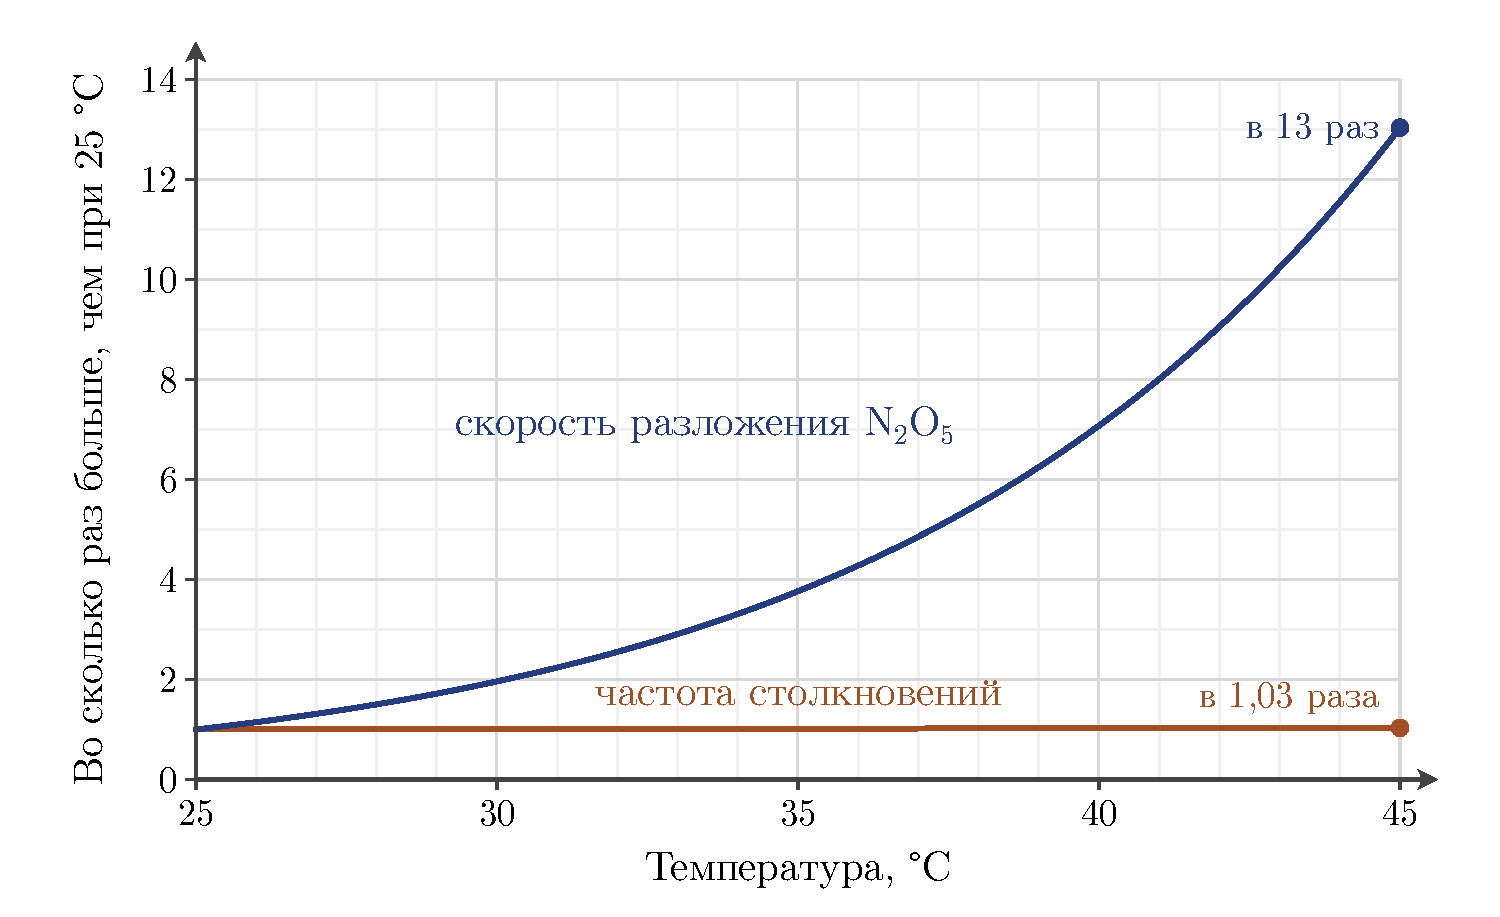
\includegraphics[width=12cm]{figs/what_affects_reaction_rate/temperature_vs_collisions.pdf}
    \caption{Во сколько раз при нагревании выше \qty{25}{\degreeCelsius} растёт скорость реакции разложения \ce{N2O5} в сравнении с частотой столкновений молекул. Скорость рассчитана по данным Эйринга и Даниэлса.}
    \label{fig:temperature_vs_collisions}
\end{figure}

В чём же тогда дело? Видимо, во втором множителе в выражении~\eqref{eq:collision_model}, от которого зависит скорость реакций, а именно в доле эффективных столкновений. Взгляните на рис.~\ref{fig:energy_threshold}. В реакцию могут вступить только молекулы, обладающие определённой энергией, необходимой для разрыва исходных химических связей (с энергией выше определённого порога). Особенностью распределения Максвелла~--- Больцмана является то, что при повышении температуры особенно сильно растёт число молекул с большой энергией, то есть правый <<хвост>> распределения. При этом средняя энергия молекул меняется не особенно сильно, а вот быстрых молекул, способных при ударе разорвать связи, становится во много раз больше. Поэтому при повышении температуры скорости химических реакций растут быстро. Как рассчитать долю молекул с энергией выше порога, мы узнаем в одном из следующих разделов.

\begin{figure}[htbp]
    \centering
    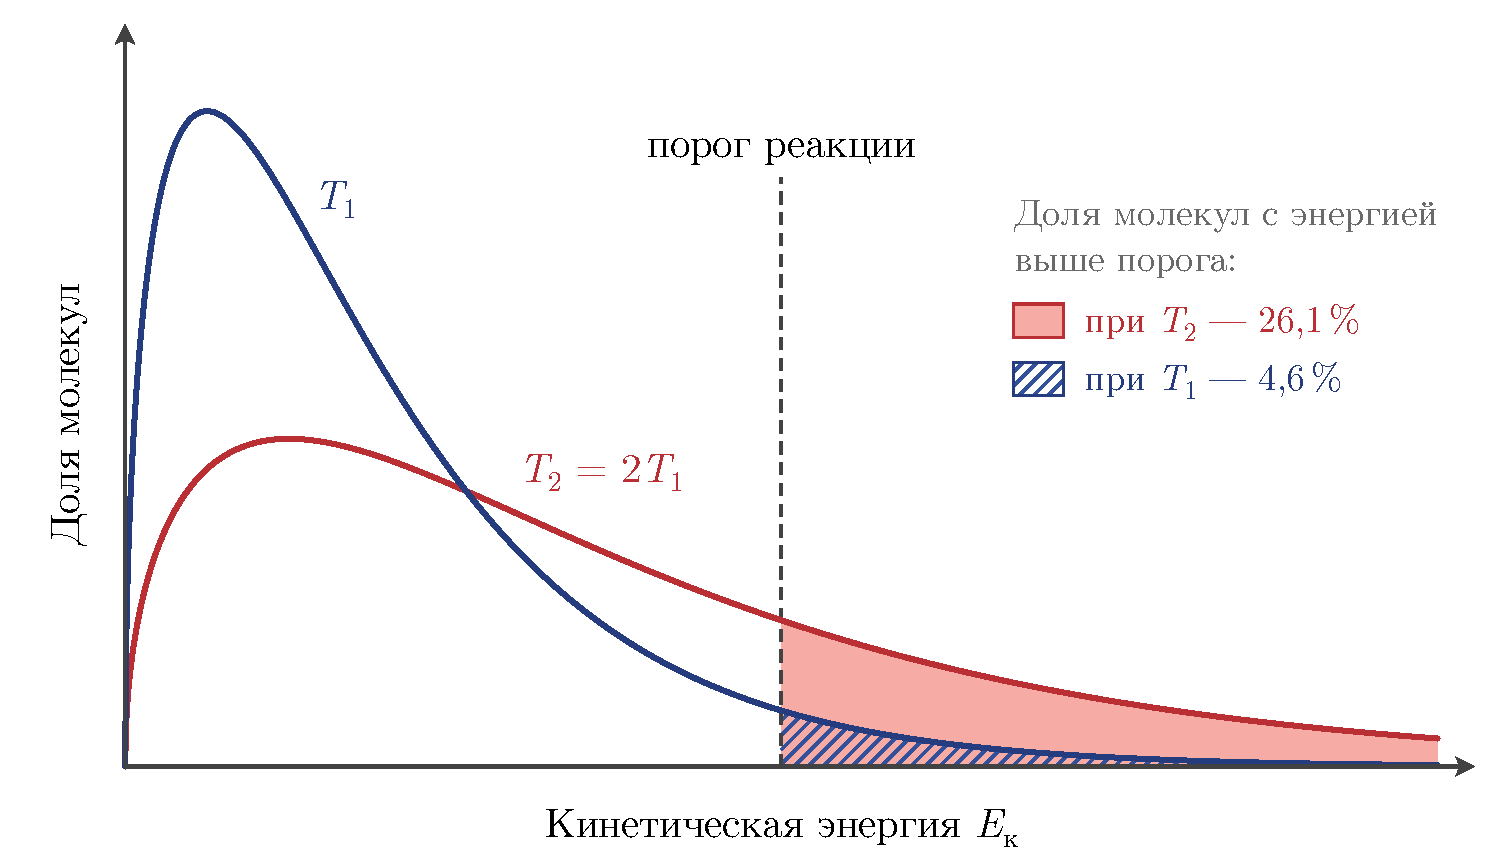
\includegraphics[width=12cm]{figs/what_affects_reaction_rate/energy_threshold.pdf}
    \caption{Доля молекул, обладающих достаточной энергией для начала реакции при температурах $T_1$ и $T_2=2T_1$. Порог для наглядности взят низким ($4kT_1$). У реальных реакций он обычно в десятки раз больше $kT$, и доля молекул больше этого порога очень мала, а при нагревании количество молекул выше порога растёт ещё сильнее.}
    \label{fig:energy_threshold}
\end{figure}

Сильное ускорение реакций при нагревании часто приводит к явлению \emph{самоподдерживания} реакций. В качестве хорошего примера можно привести обычное горение. Нам достаточно только запустить его, нагрев небольшой участок материала, после чего выделяющаяся теплота будет нагревать соседние участки, ускоряя реакцию и там. Дальше горение будет поддерживать само себя, как в эксперименте со стальной ватой, которая горела и вне пламени горелки.

\subsection*{Площадь поверхности}

В опыте №~3 и гвоздь, и стальная вата состояли из железа и контактировали с одним и тем же кислородом воздуха. Это \hyperref[term:heterogeneous_reaction]{гетерогенная реакция}, которая идёт только на границе раздела фаз, то есть на поверхности металла, а с атомами железа внутри гвоздя молекулы кислорода столкнуться не могут. Скорость гетерогенной реакции в расчёте на единицу площади определяется формулой~\eqref{eq:surface_reaction_rate} и не зависит от степени измельчения веществ. Однако очевидно, что количество вещества, которое реагирует за единицу времени, растёт вместе с площадью поверхности.

При измельчении веществ растёт именно суммарная площадь поверхности (рис.~\ref{fig:cube_division}). У кубика с ребром \qty{1}{\ruCm} площадь поверхности равна \qty{6}{\ruCm\squared}. Если мы разрежем его на 8~кубиков с ребром \qty{5}{\ruMm}, то их общая площадь станет равна \qty{12}{\ruCm\squared}. А у 1000~кубиков с ребром \qty{1}{\ruMm} она будет равна уже \qty{60}{\ruCm\squared}, то есть в десять раз больше, чем у исходного кубика, при этом масса вещества осталась прежней.

\begin{figure}[htbp]
    \centering
    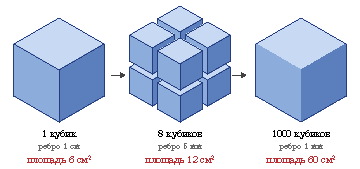
\includegraphics[width=12cm]{figs/what_affects_reaction_rate/cube_division.pdf}
    \caption{При измельчении масса вещества не меняется, а суммарная площадь поверхности растёт.}
    \label{fig:cube_division}
\end{figure}

Чтобы можно было сравнивать между собой порошки и пористые материалы, в химии используется такой показатель, как \term{удельная поверхность}{specific_surface_area}{удельная поверхность}. Она равна площади поверхности, которая приходится на единицу массы вещества:
\begin{equation}
    \label{eq:specific_surface_area}
    A_{\text{уд}} = \frac{A_{\text{пов}}}{m}.
\end{equation}
Удельную поверхность обычно выражают в \unit{\ruM\squared\per\ruG}. В нашем примере у гвоздя она составляет порядка \qty{2}{\ruCm\squared\per\ruG}, а у стальной ваты~--- порядка \qty{100}{\ruCm\squared\per\ruG}. Пористые материалы имеют поверхность не только снаружи, но и в толще материала (на стенках пор). Например, удельная поверхность активированного угля составляет от 500 до \qty{3000}{\ruM\squared\per\ruG}.

Если мы очень сильно измельчим металл, то его реакция с кислородом может ускориться настолько, что порошок будет самовоспламеняться на воздухе без поджигания. Такие вещества называют \emph{пирофорными}. Мелкий порошок железа тоже является пирофорным. При этом в виде единой массы с небольшой площадью поверхности реакция окисления железа протекает настолько медленно, что на практике гвозти могут ржаветь годами.

Однако было бы неправильно сказать, что стальная вата горит только из-за большой поверхности. Дело ещё и в том, что тонкая проволока быстро прогревается целиком, при этом выделившейся теплоте некуда уйти. А массивный гвоздь отводит теплоту от нагретого места в свою толщу и не разогревается настолько, чтобы загореться.

Для гетерогенной реакции важна именно площадь, на которой реагенты действительно соприкасаются, то есть \term{поверхность контакта}{contact_surface}{поверхность контакта}, а не просто удельная поверхность твёрдого вещества. В качестве хорошего примера можно привести муку. Мука отлично взрывается (хотя про это не все знают). Сам мешок муки, конечно, не взрывается, даже если попытаться его поджечь. Мука при этом только обгорит с поверхности. Между частицами муки в мешке, конечно, есть воздух, но кислорода в нём слишком мало, а свежий воздух внутрь почти не проникает из-за того, что частицы уложены плотно. Если же муку распылить в воздухе, то каждая её частица окажется окружена кислородом (рис.~\ref{fig:contact_surface}). В этом случае такое облако лучше не поджигать, потому что оно сгорит за доли секунду с сильным взрывом. Взвесь муки в воздухе взрывоопасна, если в кубическом метре воздуха больше примерно \qty{50}{\ruG} мучной пыли (по факту это очень густое облако).

\begin{figure}[htbp]
    \centering
    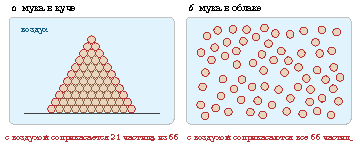
\includegraphics[width=12cm]{figs/what_affects_reaction_rate/contact_surface.pdf}
    \caption{Частицы муки: \emph{а}~--- уложенные в кучу (воздух касается только наружных частиц); \emph{б}~--- в облаке (воздух окружает каждую частицу). Частицы, соприкасающиеся с воздухом, обведены.}
    \label{fig:contact_surface}
\end{figure}

Первый зафиксированный взрыв мучной пыли произошёл в Турине в 1785~году на складе пекарни. Мука ссыпалась сверху, из-за чего поднялось облако пыли, которое вспыхнуло от лампы с открытым пламенем. Двое рабочих пострадали. В 1878~году взрыв мучной пыли разрушил в Миннеаполисе одну из крупнейших в мире мельниц, при этом погибли 18~человек. Поэтому на мельницах, элеваторах и хлебозаводах следят, чтобы мучная пыль не поднималась в воздух.

Если твёрдое вещество реагирует с раствором, то возле поверхности реагент быстро расходуется, и свежему реагенту приходится подходить из глубины раствора. При этом реакцию можно ускорить перемешиванием, которое подводит к поверхности новые порции реагента и уносит продукты. Когда мы раздуваем угли в костре, мы следуем этой самой логике, принося с потоком воздуха к поверхности углей новые порции кислорода.

\subsection*{Природа реагентов}

Давайте возьмём одинаковые по размеру кусочки магния, цинка и железа и опустим их в одну и ту же соляную кислоту (рис.~\ref{fig:metals_in_acid}). Реакция магния будет сопровождаться бурным <<вскипанием>>, цинк растворяется спокойнее, а железо~--- совсем медленно. Концентрация, температура и площадь поверхности при этом одинаковы, но скорости реакций всё равно разные, потому что разными являются сами вещества. Этот фактор называется \emph{природой реагентов} и является чрезвычайно значительным. Скорости реакций разных веществ при одних и тех же условиях могут различаться на много порядков.

\begin{figure}[htbp]
    \centering
    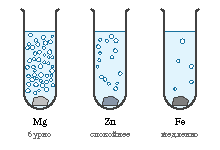
\includegraphics[width=7.33cm]{figs/what_affects_reaction_rate/metals_in_acid.pdf}
    \caption{Одинаковые кусочки магния, цинка и железа в одной и той же соляной кислоте.}
    \label{fig:metals_in_acid}
\end{figure}

Например, реакции между ионами в растворе проходят практически мгновенно (задача~\ref{prob:what_is_reaction_rate5}):
\begin{equation*}
    \ce{Ag+ + Cl- -> AgCl (v)}, \qquad \ce{H+ + OH- -> H2O}.
\end{equation*}
Для того, чтобы вступить в реакцию, ионам не нужно разрывать прочные связи, достаточно просто встретиться, чему и так способствуют противоположные заряды. Гораздо медленнее идут реакции, в которых надо разорвать прочные ковалентные связи. Смесь водорода с кислородом (энергии связей в молекулах \ce{H2} и \ce{O2} равны 436 и \qty{498}{\ruKJ\per\ruMole} соответственно) при комнатной температуре годами будет храниться без изменений. Тройная связь в молекуле азота (\qty{945}{\ruKJ\per\ruMole}) настолько прочна, что азот при обычных условиях почти ни с чем не реагирует, и аммиак из азота и водорода получают при \num{400}--\qty{500}{\degreeCelsius}, давлении в сотни атмосфер и с катализатором.

Также имеет значение строение частиц вещества. Белый фосфор, состоящий из отдельных молекул \ce{P4}, медленно окисляется на воздухе уже при комнатной температуре (из-за этого в темноте он светится зеленоватым светом), а примерно при \qty{50}{\degreeCelsius} самовоспламеняется, поэтому его хранят, залив слоем воды. Красный фосфор загорается на воздухе только при нагревании выше \qty{240}{\degreeCelsius}. Молекулы белого фосфора удерживаются друг возле друга только слабыми \hyperref[term:intermolecular_forces]{межмолекулярными силами}, поэтому часть их всегда переходит в пар и легко встречается с кислородом. В красном фосфоре атомы прочно связаны ковалентными связями в длинные цепи, и, чтобы начать реакцию, эти связи нужно разорвать.

От строения частиц также зависит, какая доля столкновений будет иметь удачную ориентацию. Ион или отдельный атом может столкнуться с партнёром любой своей стороной, а у крупной молекулы в реакцию вступает обычно лишь небольшой её участок, и удачно направленной оказывается лишь небольшая доля ударов.

\subsection*{Ещё способы управления скоростью}

Кроме концентрации, температуры, площади поверхности и природы реагентов, на скорость реакции влияют и другие факторы. Подробно мы разберём их позже, а пока познакомимся с ними на примерах.

\emph{Катализатор.} Если мы бросим в раствор пероксида водорода щепотку чёрного порошка оксида марганца (IV), раствор бурно вспенится от выделяющегося кислорода:
\reaction*{2H2O2 ->[MnO2] 2H2O + O2 (^) {.}}
Без \ce{MnO2} пероксид водорода разлагается очень медленно, а сам \ce{MnO2} после реакции остаётся в том же количестве, что и до неё. Вещества, которые ускоряют реакцию, но сами в итоге не расходуются, называют \emph{катализаторами}. В биохимических реакциях катализаторами выступают особые белки, которые называются \emph{ферментами}. Например, фермент \emph{алкогольдегидрогеназа} окисляет этанол в крови человека. Или, если налить на открытую рану раствор пероксида водорода, он вспенится, потому что будет разлагаться под действием фермента \emph{каталазы}, присутствующего в крови и тканях.

\emph{Растворитель.} В отсутствие растворителя смешанные друг с другом вещества могут реагировать очень медленно. Например, шипучие таблетки ацетилсалициловой кислоты содержат сухую смесь лимонной кислоты и гидрокарбоната натрия (питьевой соды). В упаковке она может храниться годами, но если мы растворим таблетку в воде, то эта смесь реагирует примерно за одну минуту с образованием углекислого газа, который вызывает <<вскипание>> раствора. В твёрдой смеси частицы веществ соприкасаются лишь в отдельных точках и не могут перемещаться, а в растворе молекулы и ионы свободно движутся и встречаются друг с другом. Важна также и природа самого растворителя. В конце XIX~века Николай Меншуткин обнаружил, что растворитель, сам при этом не вступая в реакцию, сильно влияет на её скорость. По современным данным, скорость изученной им реакции триэтиламина с иодэтаном в разных растворителях различается примерно в сто тысяч раз.

\emph{Излучение.} Смесь водорода с хлором в темноте может храниться долго, но стоит вам осветить эту смесь фотовспышкой, как она взорвётся. Свет обладает достаточной энергией, чтобы разорвать молекулы хлора на атомы, которые запускают цепочку быстрых превращений. С воздействием света связан и фотосинтез, и выцветание красок на солнце, и почернение фотоплёнки.

\subsection*{Подводим итоги}

Соберём все факторы в одну таблицу (табл.~\ref{tab:rate_factors}).

\begin{table}[htbp]
    \small
    \caption{Факторы, от которых зависит скорость реакции.}
    \label{tab:rate_factors}
    \begin{tabularx}{\textwidth}{
        >{\hsize=1.05\hsize}Y
        >{\hsize=0.75\hsize}Y
        >{\hsize=1.0\hsize}Y
        >{\hsize=1.2\hsize}Y
        }
        \hline
        \rowcolor{table_header}
        Фактор & Как ускорить реакцию & Почему это действует & Пример \\
        \hline
        Концентрация (для газов~--- давление) & Увеличить & Частицы чаще сталкиваются & Лучинка вспыхивает в кислороде \\
        \hline
        Температура & Повысить & Больше эффективных столкновений & Тёплый раствор тиосульфата мутнеет быстрее \\
        \hline
        Поверхность контакта & Измельчить, перемешать & Больше частиц на границе фаз & Стальная вата горит, гвоздь~--- нет \\
        \hline
        Природа реагентов & Взять другие вещества & Прочность связей, строение частиц & Белый фосфор горит легче красного \\
        \hline
        Катализатор & Добавить & Реакция идёт другим путём & \ce{MnO2} и пероксид водорода \\
        \hline
        Растворитель & Растворить реагенты & Частицы свободно движутся & Шипучая таблетка в воде \\
        \hline
        Свет & Осветить & Свет разрывает связи & Водород и хлор на свету \\
        \hline
    \end{tabularx}
\end{table}

На данном этапе мы описали действие этих факторов качественно. Но химику также нужно знать, \emph{во сколько раз} изменится скорость, если, скажем, удвоить концентрацию одного из реагентов. Для этого нам необходимо перейти к количественным закономерностям. В следующем разделе мы узнаем, как по результатам экспериментов найти зависимость скорости реакции от концентраций.

\begin{termlist}
    \hyperref[term:collision_model]{Модель столкновений},
    \hyperref[term:effective_collision]{эффективное столкновение},
    \hyperref[term:specific_surface_area]{удельная поверхность},
    \hyperref[term:contact_surface]{поверхность контакта}.
\end{termlist}

\begin{problem}{}{what_affects_reaction_rate1}
    В стакан с соляной кислотой бросили гранулу цинка. Как изменится объём водорода, выделяющегося за секунду (увеличится, уменьшится или не изменится), если:
    \begin{enumerate}[label=\arabic*)]
        \item долить в стакан равный объём воды;
        \item долить столько же кислоты той же концентрации;
        \item бросить в стакан ещё одну такую же гранулу;
        \item взять вместо гранулы цинковый порошок той же массы?
    \end{enumerate}
    Кислота взята в избытке, температура постоянна.
    \begin{sol}{\ref{prob:what_affects_reaction_rate1}}
        1)~Уменьшится. Концентрация кислоты станет вдвое меньше, и частицы кислоты будут реже сталкиваться с поверхностью цинка.

        2)~Не изменится. Скорость зависит от концентрации кислоты, а не от её количества.

        3)~Увеличится примерно вдвое, потому что вдвое вырастет площадь поверхности цинка, на которой идёт реакция. Скорость в расчёте на квадратный метр поверхности при этом не изменится.

        4)~Сильно увеличится, так как у порошка во много раз больше поверхность.
    \end{sol}
\end{problem}

\begin{problem}{}{what_affects_reaction_rate2}
    В два одинаковых стакана с равным количеством соляной кислоты бросили по \qty{1}{\ruG} \ce{CaCO3}: в первый~--- одним кусочком, во второй~--- в виде порошка. Кислота взята в избытке.
    \begin{enumerate}[label=\arabic*)]
        \item В каком стакане углекислый газ выделяется быстрее?
        \item Одинакова ли в первые секунды скорость реакции в расчёте на квадратный метр поверхности мела?
        \item В каком стакане в итоге выделится больше газа?
    \end{enumerate}
    \begin{sol}{\ref{prob:what_affects_reaction_rate2}}
        1)~Во втором. Реакция мела с кислотой гетерогенная и идёт только на поверхности мела, а у порошка поверхность гораздо больше.

        2)~Одинакова. Скорость в расчёте на единицу площади, найденная по формуле~\eqref{eq:surface_reaction_rate}, определяется условиями у поверхности, то есть концентрацией кислоты и температурой, а они в обоих стаканах одинаковы. Порошок реагирует быстрее только потому, что площадь его поверхности больше.

        3)~Одинаково. По уравнению \ce{CaCO3 + 2HCl -> CaCl2 + H2O + CO2 (^)} из \qty{1}{\ruG} карбоната кальция (\qty{0,01}{\ruMole}) образуется \qty{0,01}{\ruMole} \ce{CO2}, в какой бы форме ни был взят мел. Скорость показывает, как быстро идёт реакция, а не то, сколько получится продукта.
    \end{sol}
\end{problem}

\begin{problem}{}{what_affects_reaction_rate3}
    $\bigstar$ В опыте с тиосульфатом натрия (рис.~\ref{fig:thiosulfate_clock}) в пять стаканов налили разные объёмы $V$ раствора тиосульфата с концентрацией \qty{0,15}{\ruMolar}, долили воду до \qty{50}{\ruMl} и прилили по \qty{5}{\ruMl} соляной кислоты. Время $t$, через которое скрылся крестик, приведено в таблице.
    \begin{center}
        \small
        \begin{tabular}{cccccc}
            \hline
            \rowcolor{table_header}
            $V$, мл & 50 & 40 & 30 & 20 & 10 \\
            \hline
            $t$, с & \num{22,5} & \num{27,3} & \num{35,1} & \num{60,0} & \num{159,1} \\
            \hline
        \end{tabular}
    \end{center}
    \begin{enumerate}[label=\arabic*)]
        \item Почему величину $1/t$ можно считать мерой скорости реакции?
        \item Найдите концентрацию тиосульфата в каждом стакане после разбавления водой (до добавления кислоты) и значения $1/t$. Постройте график зависимости $1/t$ от концентрации. Пропорциональна ли скорость реакции концентрации тиосульфата?
        \item Каким было бы время для самого разбавленного раствора, если бы скорость была строго пропорциональна концентрации?
    \end{enumerate}
    \begin{sol}{\ref{prob:what_affects_reaction_rate3}}
        1)~Крестик скрывается, когда в слое раствора над ним накопится определённое количество серы. Объём раствора и высота его слоя во всех стаканах одинаковы, поэтому к моменту исчезновения крестика в каждом стакане образуется примерно одинаковое количество серы. Средняя скорость образования серы равна этому количеству, делённому на $t$, то есть пропорциональна $1/t$.

        2)~Концентрация тиосульфата после разбавления $c = \num{0,15} \cdot V/50$:

        \begin{center}
            \small
            \begin{tabular}{cccc}
                \hline
                \rowcolor{table_header}
                $V$, мл & $c$, \unit{\ruMolar} & $1/t$, \unit{\ruS\tothe{-1}} & $\dfrac{1/t}{c}$, \unit{\ruL\per\ruMole\ruS} \\
                \hline
                50 & \num{0,150} & \num{0,0444} & \num{0,30} \\
                40 & \num{0,120} & \num{0,0366} & \num{0,31} \\
                30 & \num{0,090} & \num{0,0285} & \num{0,32} \\
                20 & \num{0,060} & \num{0,0167} & \num{0,28} \\
                10 & \num{0,030} & \num{0,0063} & \num{0,21} \\
                \hline
            \end{tabular}
        \end{center}

        Для четырёх более концентрированных растворов отношение $1/t$ к концентрации почти одно и то же, около \qty{0,30}{\ruL\per\ruMole\ruS}, и точки ложатся близко к прямой, проходящей через начало координат. Значит, в этой области скорость приблизительно пропорциональна концентрации тиосульфата. А для самого разбавленного раствора отношение заметно меньше. Так что пропорциональность здесь является приближением, которое выполняется лишь в некотором интервале концентраций. У этой реакции сера образуется в несколько стадий, а крестик скрывается лишь тогда, когда её частицы вырастут до заметных размеров, так что зависимость и в самом деле сложная.

        3)~Если отношение $1/t$ к концентрации равно \qty{0,30}{\ruL\per\ruMole\ruS}, то для самого разбавленного раствора $1/t = \num{0,30} \cdot \num{0,030} = \qty{0,0090}{\ruS\tothe{-1}}$ и $t \approx \qty{110}{\ruS}$, а не \qty{159}{\ruS}.
    \end{sol}
\end{problem}

\begin{problem}{}{what_affects_reaction_rate4}
    $\bigstar$ Кубик с длиной ребра, равной $a$, разрезали на одинаковые кубики с ребром в $n$ раз меньше.
    \begin{enumerate}[label=\arabic*)]
        \item Во сколько раз выросла суммарная площадь поверхности? Проверьте ответ по рис.~\ref{fig:cube_division}.
        \item Размер частиц пшеничной муки~--- порядка \qty{50}{\ruUm}. Считая частицы кубиками, оцените, во сколько раз площадь их поверхности больше, чем у кубика с ребром \qty{1}{\ruCm} той же массы.
        \item Оцените удельную поверхность муки и площадь поверхности частиц в \qty{1}{\ruKg} муки. Плотность вещества частиц примите равной \qty{1,5}{\ruG\per\ruCm\cubed}.
    \end{enumerate}
    \begin{sol}{\ref{prob:what_affects_reaction_rate4}}
        1)~Получится $n^3$ кубиков, площадь поверхности каждого равна $6(a/n)^2$, а суммарная площадь
        \begin{equation*}
            n^3 \cdot 6\left(\frac{a}{n}\right)^2 = n \cdot 6a^2,
        \end{equation*}
        то есть она выросла в $n$ раз. На рис.~\ref{fig:cube_division} при $n = 2$ площадь выросла с 6 до \qty{12}{\ruCm\squared}, а при $n = 10$~--- до \qty{60}{\ruCm\squared}.

        2)~Ребро уменьшилось в $n = \qty{1}{\ruCm}/\qty{50}{\ruUm} = \qty{10000}{\ruUm}/\qty{50}{\ruUm} = 200$~раз, во столько же раз выросла и площадь.

        3)~У кубика с ребром $a$ площадь поверхности $6a^2$, а масса $\rho a^3$, поэтому по формуле~\eqref{eq:specific_surface_area}
        \begin{equation*}
            A_{\text{уд}} = \frac{6a^2}{\rho a^3} = \frac{6}{\rho a} = \frac{6}{\qty{1,5}{\ruG\per\ruCm\cubed} \cdot \qty{5e-3}{\ruCm}} = \qty{800}{\ruCm\squared\per\ruG} = \qty{0,08}{\ruM\squared\per\ruG}.
        \end{equation*}
        У частиц в \qty{1}{\ruKg} муки площадь поверхности около \qty{80}{\ruM\squared}, это площадь пола небольшой квартиры.
    \end{sol}
\end{problem}

\begin{problem}{}{what_affects_reaction_rate5}
    Профессор Недоумелкин объясняет студентам: <<При нагревании на \qty{10}{\degreeCelsius} молекулы начинают двигаться быстрее и потому чаще сталкиваются. Вот почему скорость реакции вырастает в 2--4~раза>>. Проверьте его объяснение: во сколько раз увеличивается скорость движения молекул газа, а значит, и частота их столкновений, при нагреве от 20 до \qty{30}{\degreeCelsius}? В чём ошибка профессора?
    \begin{sol}{\ref{prob:what_affects_reaction_rate5}}
        Скорость движения молекул пропорциональна квадратному корню из абсолютной температуры, поэтому
        \begin{equation*}
            \frac{\upsilon_2}{\upsilon_1} = \sqrt{\frac{T_2}{T_1}} = \sqrt{\frac{303}{293}} \approx \num{1,017}.
        \end{equation*}
        Частота столкновений вырастет всего на \qty{1,7}{\percent}, а не в 2--4~раза. Профессор отчасти прав, потому что столкновения действительно учащаются, но этот вклад незначителен. При нагревании значительно увеличивается количество молекул с большой энергией (правого <<хвоста>> распределения Максвелла~--- Больцмана), а значит, и доли эффективных столкновений, которые могут разорвать связи.
    \end{sol}
\end{problem}

\begin{problem}{}{what_affects_reaction_rate6}
    В медицинском кислородном баллоне газ находится под давлением около \qty{150}{\ruBar}. Во сколько раз концентрация кислорода в баллоне больше, чем в атмосферном воздухе, где парциальное давление кислорода составляет около \qty{0,21}{\ruBar}? Температуру считайте одинаковой, а газ~--- идеальным. Почему вентили и редукторы кислородных баллонов категорически запрещено смазывать маслом?
    \begin{sol}{\ref{prob:what_affects_reaction_rate6}}
        При одинаковой температуре концентрация газа пропорциональна его парциальному давлению:
        \begin{equation*}
            \frac{c_{\text{баллон}}}{c_{\text{воздух}}} = \frac{150}{\num{0,21}} \approx 700.
        \end{equation*}
        Минеральные масла и смазки самовоспламеняются в сжатом кислороде уже при температурах около \qty{200}{\degreeCelsius}. Такой нагрев может произойти при резком открывании вентиля, когда кислород в редукторе за доли секунды сжимается от атмосферного давления до \qty{150}{\ruBar} и нагревается (как воздух в велосипедном насосе, только на сотни градусов). Вспыхнувшее масло поджигает уплотнения, а затем и металлические детали, которые в чистом кислороде тоже горят. Поэтому кислородные вентили открывают медленно, а смазывают их только специальными фторированными смазками, которые воспламеняются в кислороде лишь выше \qty{400}{\degreeCelsius}.
    \end{sol}
\end{problem}

\begin{problem}{}{what_affects_reaction_rate7}
    Ржавление~--- это реакция железа с кислородом, для которой необходима вода. Предложите способы замедлить ржавление стальных инструментов, которые хранятся в гараже. Для каждого способа укажите, на какой фактор он действует.
    \begin{sol}{\ref{prob:what_affects_reaction_rate7}}
        Можно предложить, например, следующие способы.
        \begin{itemize}
            \item Хранить инструменты сухими, в ящике с влагопоглотителем, например силикагелем. Без воды реакция почти не будет протекать (при относительной влажности воздуха ниже примерно \qty{60}{\percent} чистая сталь практически не ржавеет). В этом способе мы уменьшаем концентрацию одного из реагентов.
            \item Покрыть инструменты тонким слоем масла, воска или краски. Покрытие отделяет металл от воздуха и воды, то есть уменьшает поверхность контакта.
            \item Смыть с инструментов соль и грязь. Соль с зимних дорог и грязь удерживают на металле влагу и ускоряют ржавление.
            \item Счистить уже появившуюся ржавчину. Она рыхлая, не защищает металл и удерживает воду.
            \item Избегать резких перепадов температуры, чтобы избежать выпадения конденсата на инструментах.
        \end{itemize}
        Кроме того, существуют ингибиторы коррозии~--- вещества, которые замедляют ржавление. О них мы поговорим позже.
    \end{sol}
\end{problem}

\clearpage